%% 
%% Copyright 2007, 2008, 2009 Elsevier Ltd
%% 
%% This file is part of the 'Elsarticle Bundle'.
%% ---------------------------------------------
%% 
%% It may be distributed under the conditions of the LaTeX Project Public
%% License, either version 1.2 of this license or (at your option) any
%% later version.  The latest version of this license is in
%%    http://www.latex-project.org/lppl.txt
%% and version 1.2 or later is part of all distributions of LaTeX
%% version 1999/12/01 or later.
%% 
%% The list of all files belonging to the 'Elsarticle Bundle' is
%% given in the file `manifest.txt'.
%% 

%% Template article for Elsevier's document class `elsarticle'
%% with numbered style bibliographic references
%% SP 2008/03/01

\documentclass[preprint,1p]{elsarticle}
\biboptions{numbers,sort&compress}

%% Use the option review to obtain double line spacing
%% \documentclass[authoryear,preprint,review,12pt]{elsarticle}

%% Use the options 1p,twocolumn; 3p; 3p,twocolumn; 5p; or 5p,twocolumn
%% for a journal layout:
%% \documentclass[final,1p,times]{elsarticle}
%% \documentclass[final,1p,times,twocolumn]{elsarticle}
%% \documentclass[final,3p,times]{elsarticle}
%% \documentclass[final,3p,times,twocolumn]{elsarticle}
%% \documentclass[final,5p,times]{elsarticle}
%% \documentclass[final,5p,times,twocolumn]{elsarticle}

%% For including figures, graphicx.sty has been loaded in
%% elsarticle.cls. If you prefer to use the old commands
%% please give \usepackage{epsfig}

%% The amssymb package provides various useful mathematical symbols
\usepackage{amssymb}
\usepackage{lineno}
\usepackage{hyperref}

%% The amsthm package provides extended theorem environments
%% \usepackage{amsthm}

%% The lineno packages adds line numbers. Start line numbering with
%% \begin{linenumbers}, end it with \end{linenumbers}. Or switch it on
%% for the whole article with \linenumbers.
%% \usepackage{lineno}

%% Title, authors and addresses
%% use the tnoteref command within \title for footnotes;
%% use the tnotetext command for theassociated footnote;
%% use the fnref command within \author or \address for footnotes;
%% use the fntext command for theassociated footnote;
%% use the corref command within \author for corresponding author footnotes;
%% use the cortext command for theassociated footnote;
%% use the ead command for the email address,
%% and the form \ead[url] for the home page:
%% \title{Title\tnoteref{label1}}
%% \tnotetext[label1]{}
%% \author{Name\corref{cor1}\fnref{label2}}
%% \ead{email address}
%% \ead[url]{home page}
%% \fntext[label2]{}
%% \cortext[cor1]{}
%% \address{Address\fnref{label3}}
%% \fntext[label3]{}


\journal{Nucl. Instrum. Meth. A}

\begin{document}
  
%\maketitle
%\flushbottom
\linenumbers

\begin{frontmatter}

\title{Precision Timing Detectors with Cadmium-Telluride Sensor}


\author[1]{A.~Bornheim}
\author[1]{C.~Pena}
\author[1]{M.~Spiropulu}
\author[1]{S.~Xie\corref{cor}}
\ead{sixie@hep.caltech.edu}
\author[1]{Z.~Zhang}
\address[1]{California Institute of Technology, Pasadena, CA, USA}
\cortext[cor]{Corresponding author}


\begin{abstract}
Precision timing detectors for high energy physics experiments with temporal resolutions of a few $10$~ps are
of pivotal importance to master the challenges posed by the highest energy particle accelerators such as the LHC.
Calorimetric timing measurements have been a focus of recent research, enabled by exploiting the temporal 
coherence of electromagnetic showers. Scintillating crystals with high light yield as well as silicon sensors
are viable sensitive materials for sampling calorimeters. Silicon sensors have very high efficiency for 
charged particles. However, their sensitivity to photons, which comprise a large fraction of the
electromagnetic shower, is limited. To enhance the efficiency of detecting photons, materials with higher atomic numbers than silicon 
are preferable.  In this paper we present test beam measurements with a Cadmium-Telluride (CdTe) sensor as 
the active element of a secondary emission calorimeter with focus on the timing performance of the detector. 
A Schottky type CdTe sensor with an active area of $1$~$\mathrm{cm}^{2}$ and a thickness of $1$~mm 
is used in an arrangement with tungsten and lead absorbers. Measurements are performed with electron beams 
in the energy range from 2 GeV to 200 GeV. A timing resolution of 25 ps is achieved under the best conditions.
\end{abstract}

\begin{keyword}
Cadmium Telluride \sep Timing \sep Calorimeter
\end{keyword}

\end{frontmatter}

%% \linenumbers
%
%% main text
%
\section{Introduction} 

There has been much recent interest in highly granular calorimeters with 
precision timing capability at the level of $20-30$~ps in light of the High-Luminosity
LHC and future higher energy hadron colliders. In order to probe increasingly
rare interactions, future hadron colliders must provide large 
instantaneous luminosity well above $10^{35}$~$\mathrm{cm}^{-2}\mathrm{s}^{-1}$.
With current accelerator and particle detector capabilities, such a high 
instantaneous luminosity will result in very large amounts
of pileup, exceeding several hundreds of simultaneous inelastic collisions per
bunch crossing. Therefore, the crucial ability to identify the origin 
of the particles produced at the different interaction points will be severely 
degraded. Precision timing detectors can be used to recover the ability to 
discriminate between particles produced by different inelastic collisions.
For beam bunch profiles similar to that of the LHC, a detector 
that can measure the time of arrival of a particle
with a precision of $20-30$~ps can effectively reduce the impact of
pileup by a factor of $5$ to $10$. 

Highly granular calorimeters based on silicon sensors as the active material 
have been the focus of recent interest~\cite{Adloff:2009,Butler:2020886}, due to
radiation hardness considerations as well as maturity of the silicon sensor
technology. In this article, we present results of studies of a 
calorimeter prototype using Cadmium-Telluride (CdTe) sensors as the 
active material. CdTe has been studied extensively in the context
of thin film solar cells and has become a mature and wide-spread
technology~\cite{cdtegeneric}. It has also been used as a radiation
detector for nuclear spectroscopy, and is known to have high
quantum efficiency for photons in the x-ray range of the 
spectrum~\cite{cdtesensorsgeneric,cdtesensors1,cdtesensors2,cdtesensors3}.
This feature is of particular interest in the context of its use
in calorimetery because it would be uniquely sensitive to secondary
electromagnetic shower particles in the keV range. Conventional prototypes 
using silicon or scintillator material are not directly sensitive to such high 
energy shower secondaries. Therefore, the first study of electromagnetic
showers using CdTe sensors has the potential to yield new insight
into the behavior of secondary particles produced within an 
electromagnetic shower with energies in the keV range, and has the potential
to yield an improvement on the energy measurement due to
the additional contribution of the higher energy x-ray photons to which previous
calorimeters were not sensitive.

The recent interest on precision timing has resulted in new studies of 
the timing properties of silicon sensors. These studies have found a time resolution 
at $20$~ps level, provided a sufficiently large signal size
in a variety of applications ranging from calorimetery~\cite{SiliconTiming} to 
charged particle detectors~\cite{santacruz}. The signal formation process
in CdTe sensors are very similar to the process in silicon and has 
similar potential to yield precise timestamps.

In this article, we study the signal response of the CdTe sensor to electromagnetic
showers of varying energies and at different shower depths. We also study the timing
performance of the CdTe sensors for electromagnetic showers.


%
%
%
%
%
\section{Cadmium Telluride Sensor}
\label{sec:siliconpad}
%Fig: Quantum Efficiency vs wavelength
%Photos of sensor, drawing for the circuit
The semi-conducting properties of Cadmium-Telluride has been studied since many decades~\cite{cdtegeneric}, 
in particular in the the context of using the material in photovoltaic applications.
Cadmium-telluride sensor are widely used in X-ray detectors~\cite{cdtesensorsgeneric,cdtesensors2,cdtesensors3}. 
They have also been investigated for synchrotron radaition detectors in accelerator technology~\cite{cdtelhc}.   
In our previous 
studies~\cite{Anderson:2015gha,MCPShowerMaxPaper,Ronzhin201552,SiliconTiming,PixelatedMCP,Anderson:2016ygg,Anderson:2015tia} 
we have demonstrated that increasing the primary sensor signal is crucial to achieve good timing resolutions.  
Cadmium-telluride features a significantly larger efficiency for detecting photons in the $10-100$~keV energy range 
compared to silicon sensors. The higher atomic number of Cadmium and Tellurium, averaging to 48.52 for the 
compound bulk material, results in a higher interaction cross section for photons in this energy range. 
Photons with such energies are abundant in electromagnetic showers~\cite{showercomposition}. 
Furthermore, CdTe sensor are available with thicknesses of $1$~mm and more. 
The path-length of the charged shower particles in the sensor material scales accordingly, 
resulting in a larger primary signal.
%
Our measurements were conducted with a CdTe Schottky type diode purchased from Acrorad~\cite{acrorad}. 
It is $1$~$\mathrm{cm}^{2}$ in transverse size and $1$~mm thick.
It was operated at a bias voltage of $700$~V and the dark current was between $3$~nA 
and $6$~nA depending on the environmental conditions in the test beam experimental 
zones.     
%
\begin{figure}[htbp] 
\centering
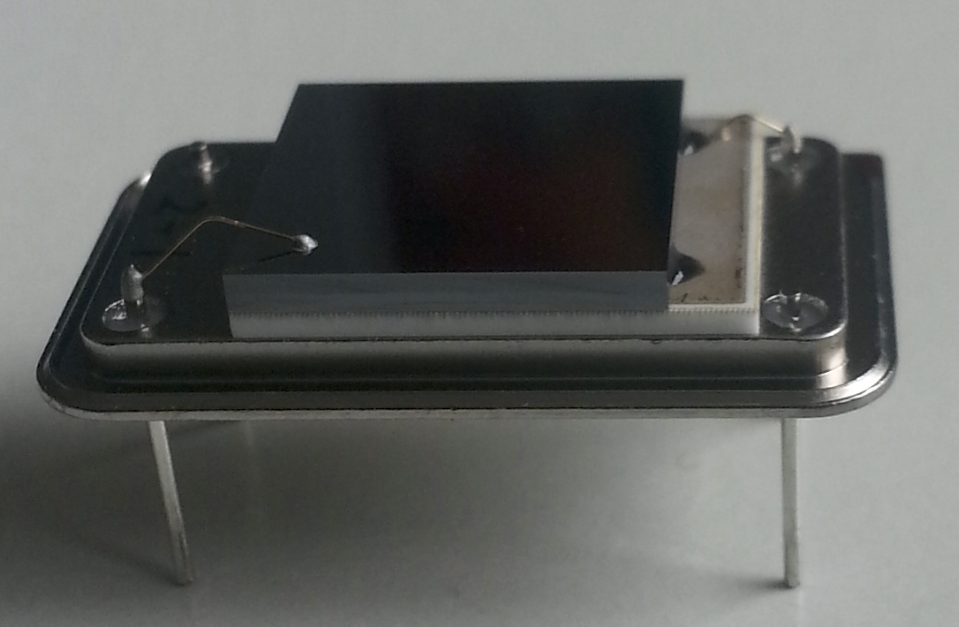
\includegraphics[width=0.55\textwidth]{figures/CdTeSensor.png} 
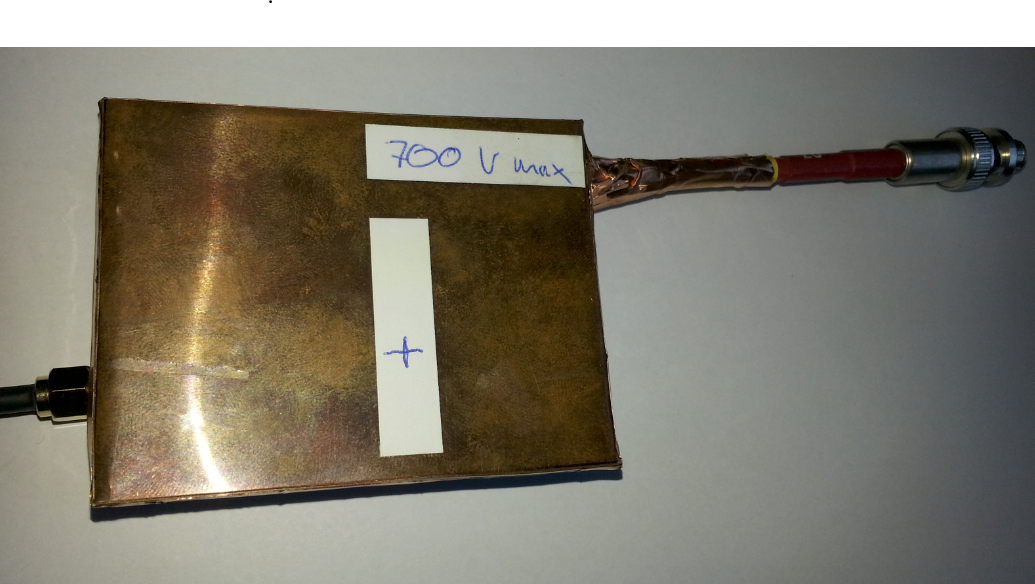
\includegraphics[width=0.37\textwidth]{figures/CdTeSensorBox.png} 
\caption{Left: CdTe sensor used in the setup. The sensor is a Schottky type diode with a transverse size 
of $1$~$\mathrm{cm}^{2}$ and a thickness of $1$~mm. It is biased at $700$~V. 
On the front, left corner of the sensor the wire bond connection 
to the metalized top layer of the sensor can be seen. Right: A photograph of the copper box
enclosing the CdTe sensor. } 
\label{fig:CdTeSensor} 
\end{figure} 
%
The sensor was placed in a box made of $0.3$~mm aluminium sheets sealed with copper tape. 
The electrical circuit shown in Fig.~\ref{fig:cdtecircuit} was used to connect to the sensor to the bias 
voltage with a standard high voltage cable and the readout electronics using a SMA cable with a feed 
through penetrating the aluminium box.

%
\begin{figure}[htbp] 
\centering
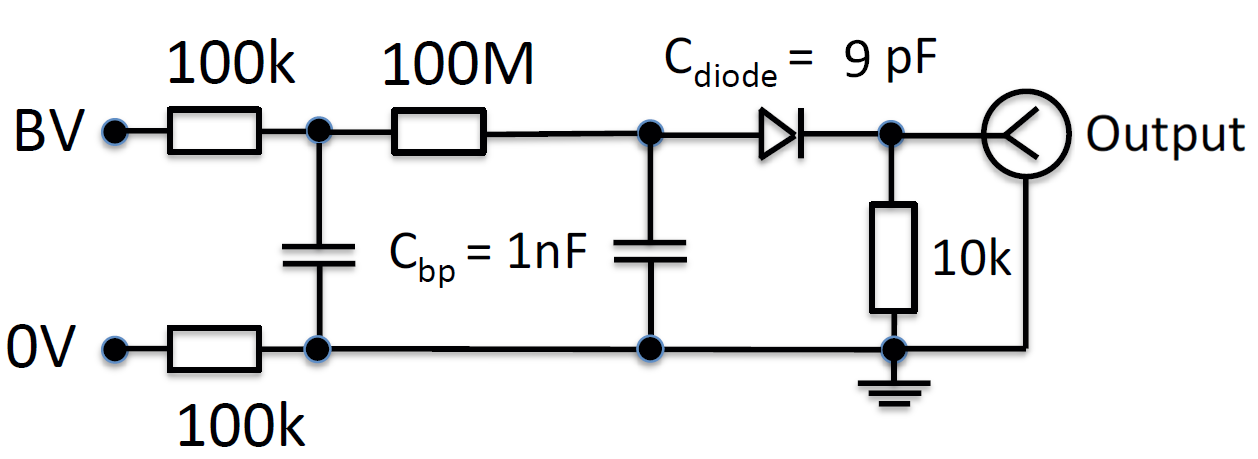
\includegraphics[width=0.49\textwidth]{figures/circuit_CdTe.png} 
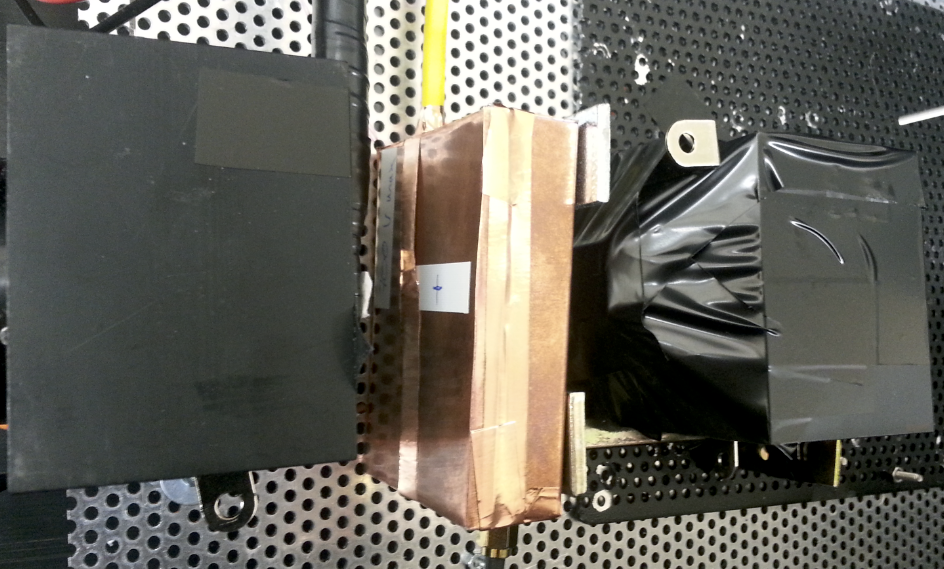
\includegraphics[width=0.49\textwidth]{figures/CdTeT9Setup.png} 
\caption{Schematic diagram of the circuit used to polarize and read out the 
CdTe sensor. The circuit and the sensor are enclosed in a copper box. Right : Setup in the T9 beam line with the reference timing MCP to the left, followed to the right by a scintillator counter, the copper box with the CdTe sensor and an MCP with a LYSO cube mounted onto it.} 
\label{fig:cdtecircuit} 
\end{figure} 
%
  
%
%
\section{Test-beam Setup and Experimental Apparatus }
\label{sec:tbeam}

We performed the measurements at the H2 beamline of the CERN North-Area testbeam facility
and the T9 beamline of the CERN East-Area testbeam facility. They provide electron beams 
from the Proton Synchrotron (PS) and Super Proton Synchrotron (SPS)
of energies ranging from $2$~GeV to $200$~GeV. The beams are composed of 
a mixture of electrons and pions. The electron fraction in the beam at H2 is typically larger than 75\%
while at T9 it is typically about 10\%. 

Trigger counters made of photomultipliers coupled to $4$~$\mathrm{cm}$~$\times$~$4$~$\mathrm{cm}$ 
plastic scintillators are used 
to initiate the read out of the data acquisition (DAQ) system. The DAQ system
uses a CAEN V1742 switched capactor digitizer based on the DRS4 chip~\cite{DRS4}. Wire chambers
are used to measure the position of each incident beam particle in the plane transverse
to the beamline. A stack of lead or tungsten absorbers of different thicknesses are 
placed about $5$~mm in front of the CdTe sensor, which is 
enclosed within a copper box. We amplified the size of the
signals from the CdTe sensor using a Hamamatsu C5594 amplifier~\cite{HamaAmpDataSheet} with a bandwidth of
$1.5$~GHz and providing a voltage gain of $36$~dB. A $10$~dB attenuator was used to attenuate the input signal 
to the amplifier for beam energies of 50 GeV and above to adjust the CdTe signal to the dynamic range of the amplifier. 
A micro-channel plate photomultiplier (MCP-PMT)
detector is used to provide a very precise reference timestamp. At the T9 beamline,
a Hamamatsu R3809U MCP-PMT~\cite{HamaMCPDataSheet} is placed just upstream of the absorber material. 
At the H2 beamline a Photek 240 MCP-PMT~\cite{PhotekDataSheet} is used, which contains a significant 
amount of absorber material (about 1.8 radiation lengths), and is therefore placed 
just downstream of the CdTe sensor to avoid inducing an early electromagnetic shower.
The precision of the time measurement for both types of MCP-PMTs is less than 
$10$~ps~\cite{MCPShowerMaxPaper,Anderson:2015gha}. As the purity of the electron beam at the T9 beamline is
significantly lower than at the H2 beamline, we use a LYSO crystal
optically coupled to an MCP-PMT as a means of discriminating the electrons from the pions
in the beam. The entire setup of absorber, reference counter and CdTe sensor box is housed in an aluminum
box to provide further shielding against environmental noise.
The schematic diagrams of the experimental setups at H2 and T9 
are shown in Figure~\ref{fig:BeamSchematicDiagram}, and a photograph
of the contents of the aluminum box for the setup at T9 is shown in 
Figure~\ref{fig:SetupPhoto}.


%Fig: Diagram of detector elements
\begin{figure}[htbp] 
\centering
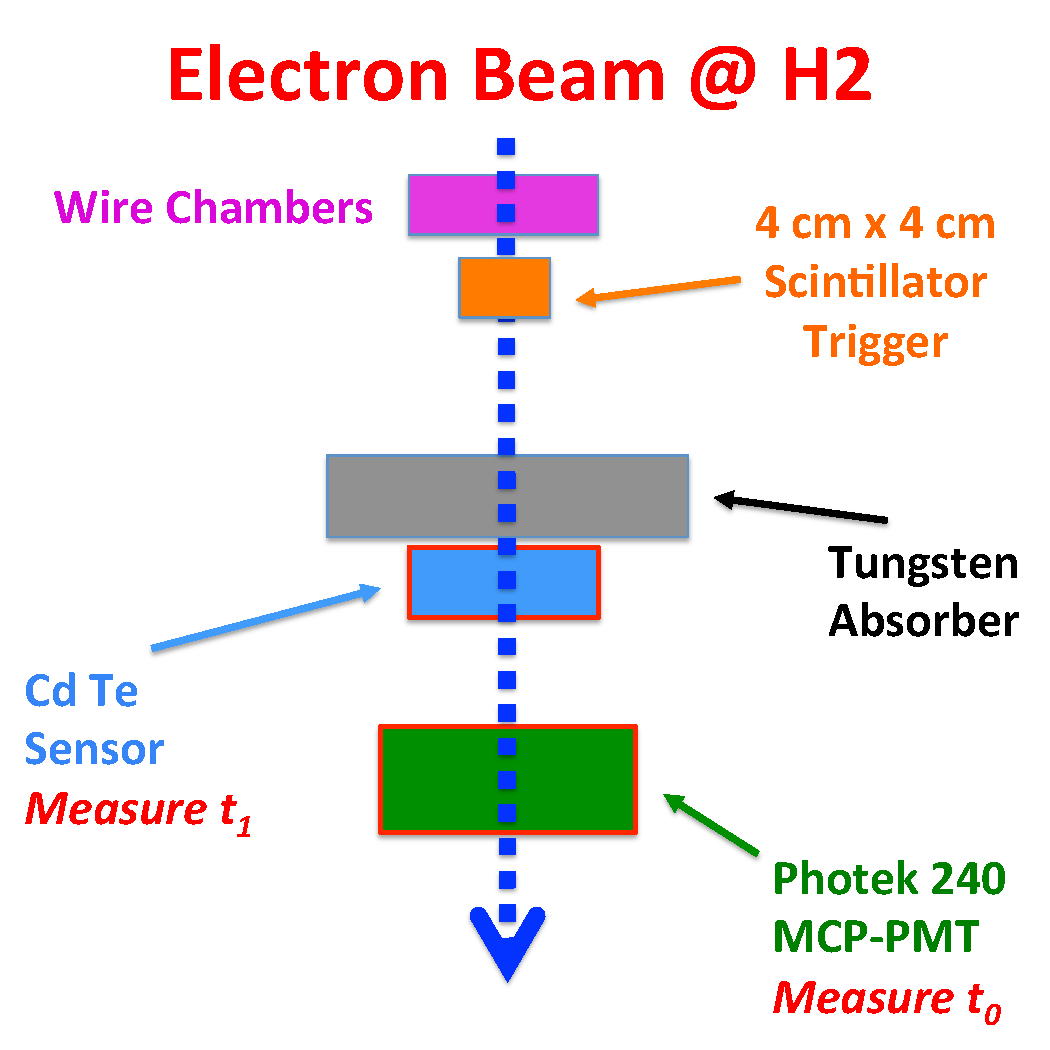
\includegraphics[width=0.49\textwidth]{figures/H2_BeamSchematicDiagram.pdf} 
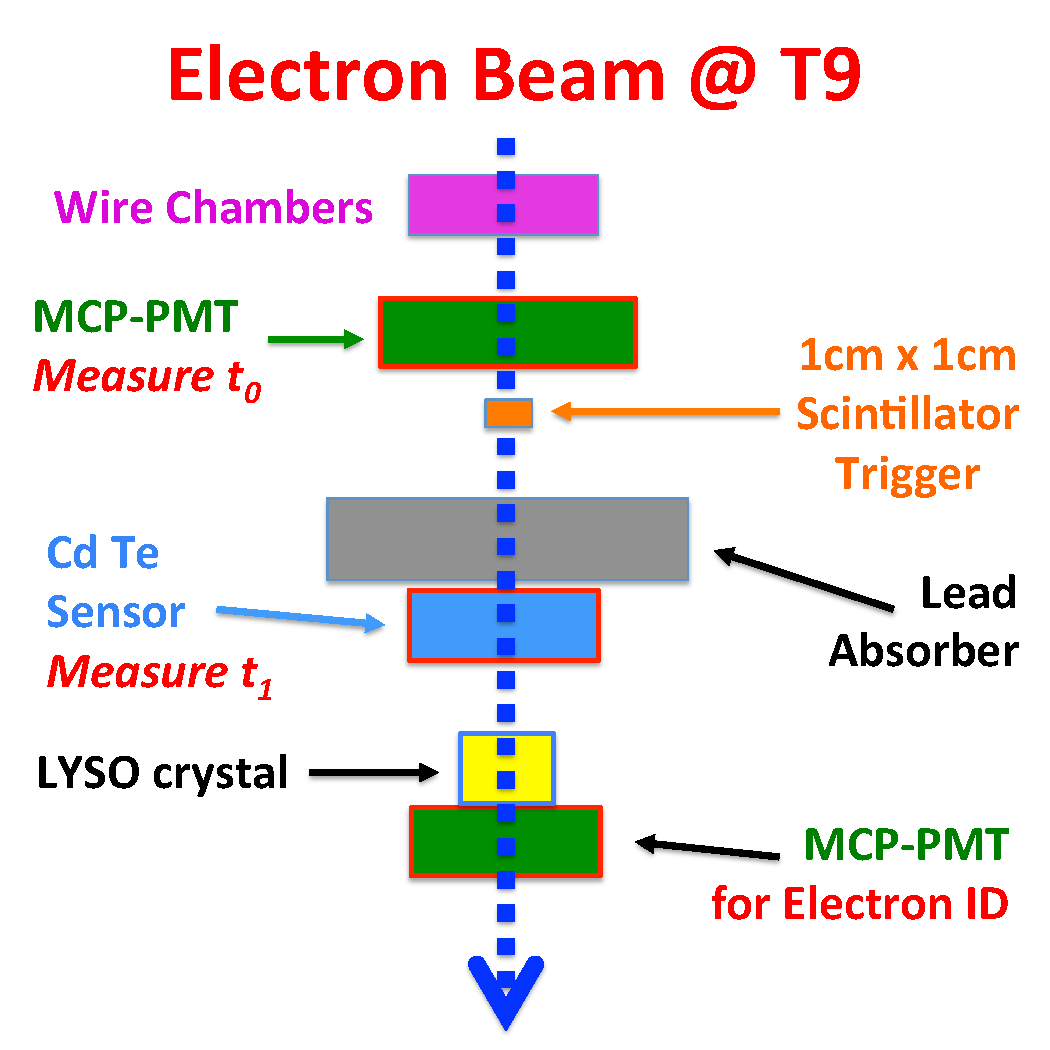
\includegraphics[width=0.49\textwidth]{figures/T9_BeamSchematicDiagram.pdf} 
\caption{Schematic diagrams of the test-beam setups at H2 (left) and T9 (right) are shown. 
The timestamps $t_0$ and $t_1$ are defined in Section~\ref{sec:reco}.} 
\label{fig:BeamSchematicDiagram} 
\end{figure} 

\begin{figure}[htbp] 
\centering
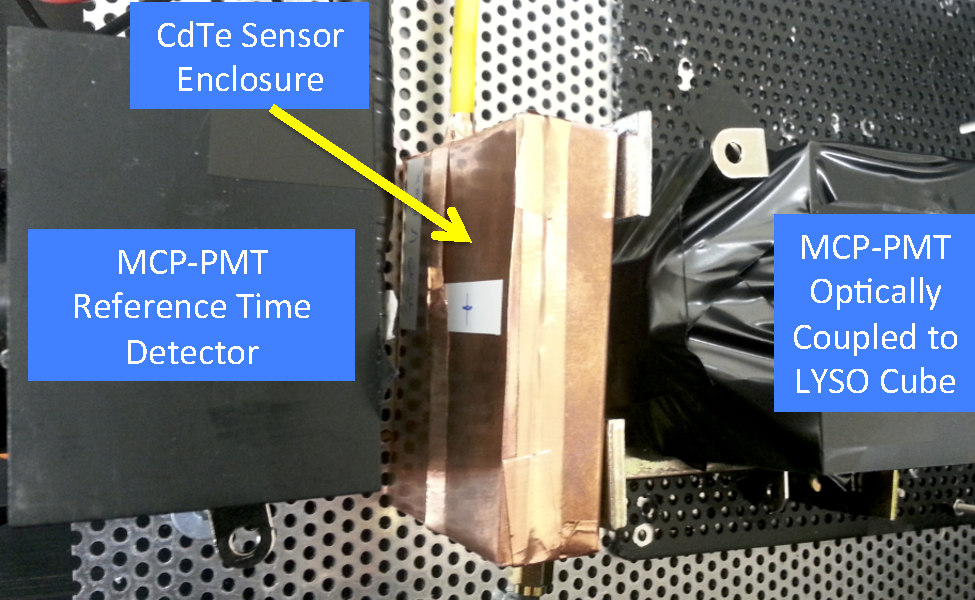
\includegraphics[width=0.75\textwidth]{figures/T9SetupPhoto.pdf} 
\caption{ Photograph of the setup used in the T9 beam line. The reference timing MCP-PMT 
is located on the leftmost region of the photo, followed to the right by a scintillator counter, 
the copper box enclosing the CdTe sensor and an MCP-PMT optically coupled to a LYSO cube. 
The lead absorber is not present in the photo and was later inserted in front of the copper box.} 
\label{fig:SetupPhoto} 
\end{figure} 


The horizontal and vertical position measurements from the wire chamber are used to determine the location
of the CdTe sensor relative to the beam and to align the beam. In 
Figure~\ref{fig:BeamSensorPosition}, we show the average amplitude measured in the
CdTe sensor as a function of the horizontal and vertical positions as measured by the wire chamber. Based
on these plots, we can restrict our measurements to those electrons whose impact point is close
to the center of the CdTe sensor.

%Fig: Beam profile X-Y plot
\begin{figure}[htbp] 
\centering
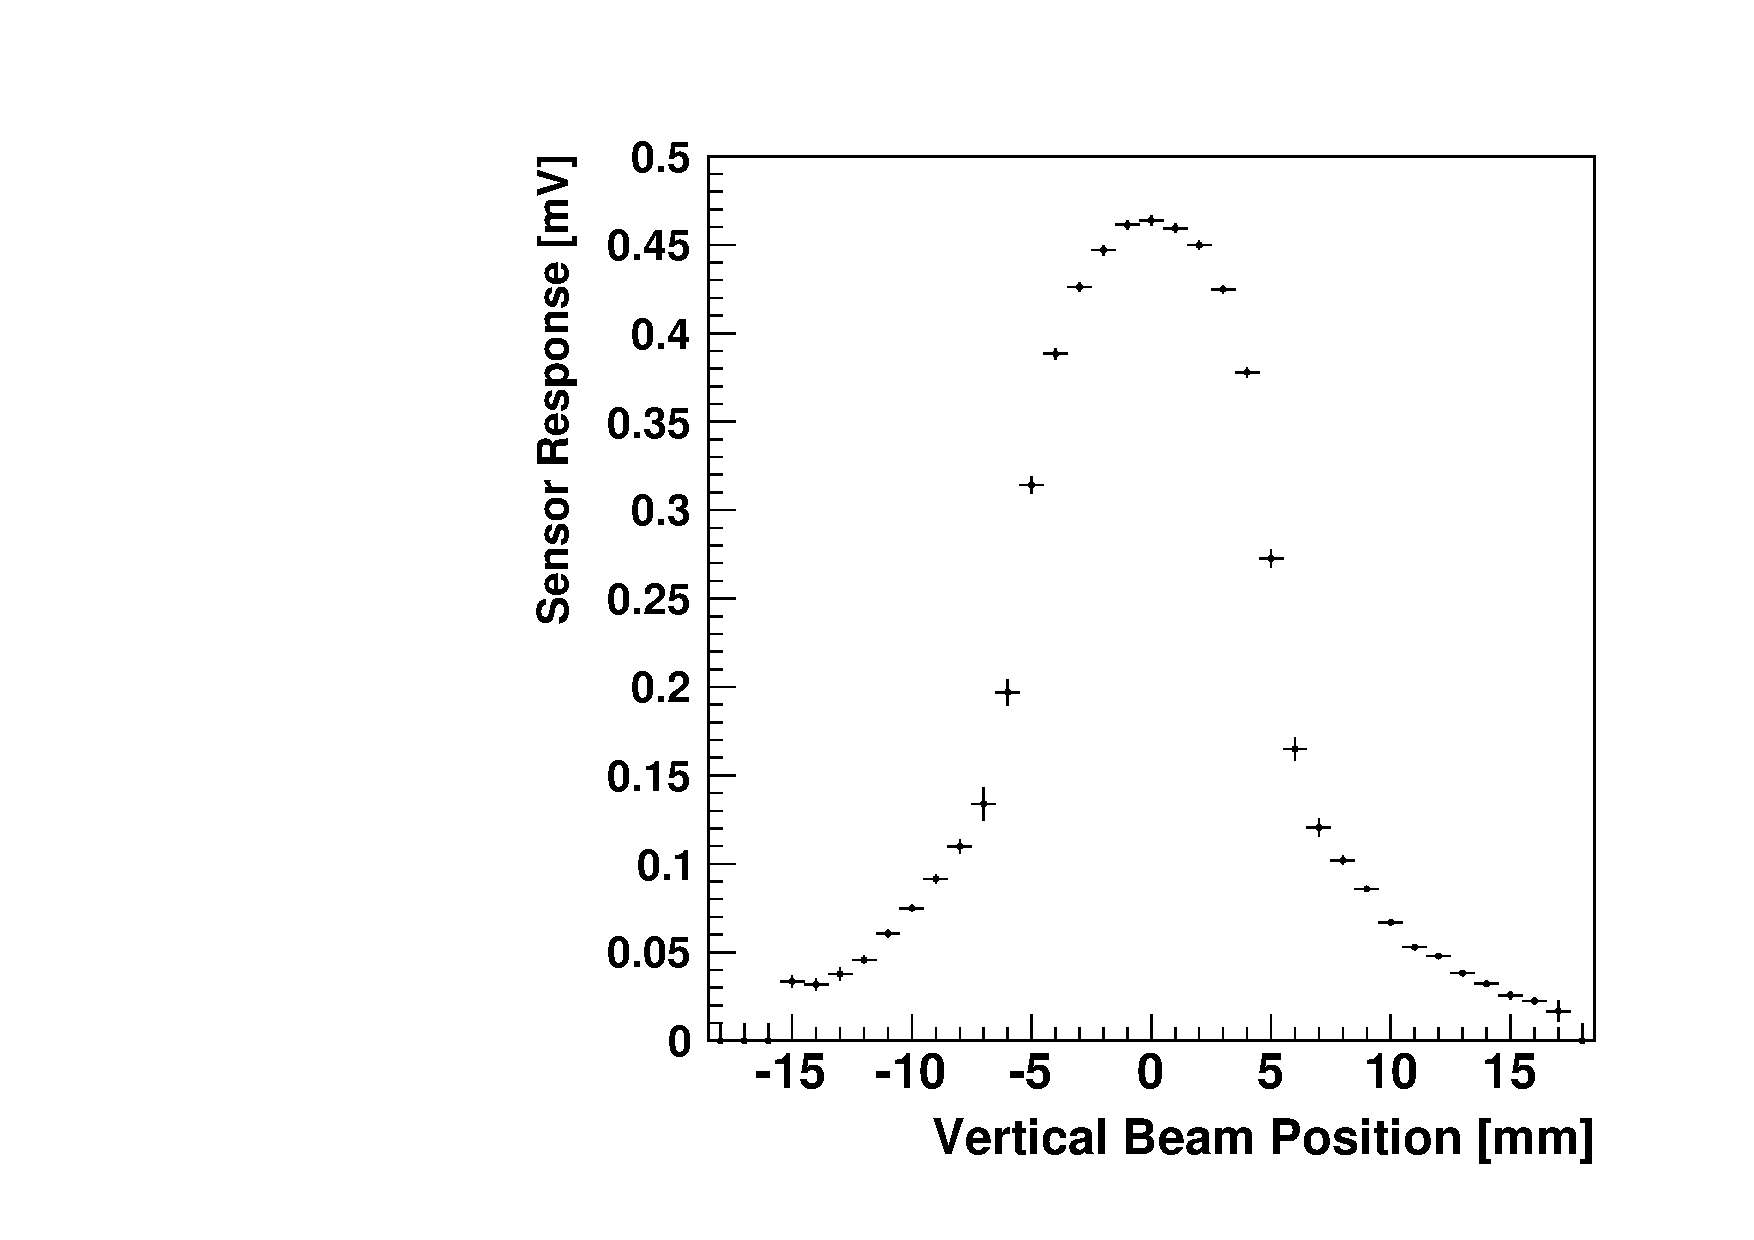
\includegraphics[width=0.49\textwidth]{figures/CdTeProfile_X.pdf} 
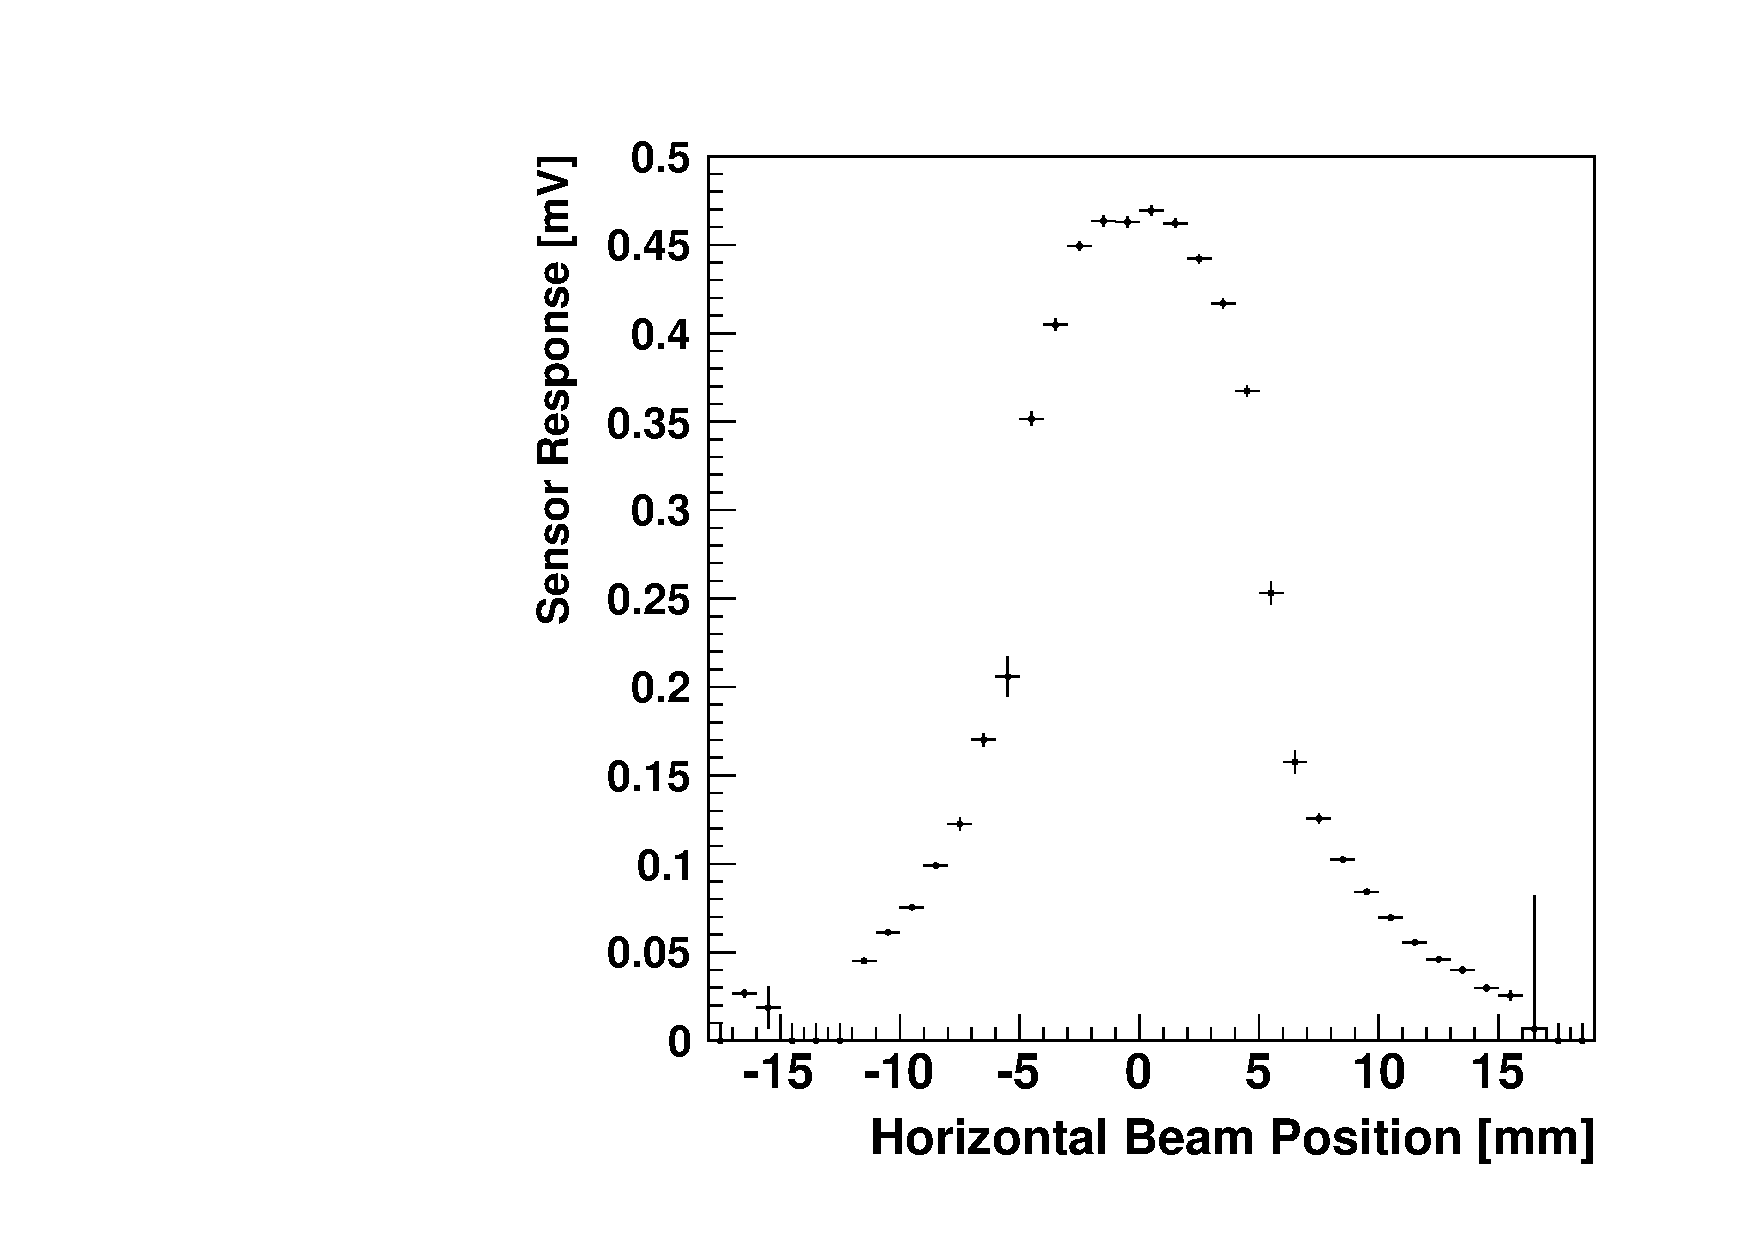
\includegraphics[width=0.49\textwidth]{figures/CdTeProfile_Y.pdf} 
\caption{The average amplitude measured in the CdTe sensor is plotted as a function of 
the horizontal and vertical positions of the beam particle as measured by the wire chamber. The measurement shown was performed with electrons of 100 GeV and $6\, X_0$ of absorber.} 
\label{fig:BeamSensorPosition} 
\end{figure} 

  
%
%

\section{Event Reconstruction and Selection }
\label{sec:reco}

All signals are recorded by the CAEN V1742 digitizer with a sampling time of $200$~ps.
The baseline pedestal for each channel is determined using the time samples outside of
the signal window, and is subsequently subtracted from the signal pulses. An example of a recorded
signal waveform in the CdTe sensor for an electromagnetic shower from a 100 GeV electron is shown 
in Figure~\ref{fig:Pulses}. We did not observe an obvious energy dependency of the pulse shapes on 
the particle energy. The pulses feature two components, an initial faster one lasting about 10 ns 
followed by a component extending slightly beyond the 200 ns time window of our readout system. 
The drift velocity of electrons in CdTe is known to be much higher than for the 
holes \cite{scpulses}, which may cause such a pulse shape. The relative size of 
the two signal components are observed to be independent of the energy of the 
incident electron, and therefore its energy may be determined from the fast 
component alone. Using randomly triggered data, we measured the RMS of 
the noise for the channel reading out the CdTe sensor after the amplifier to be about $1.3$~mV. 

%Fig: Pulse shapes for various energies
\begin{figure}[htbp] 
\centering
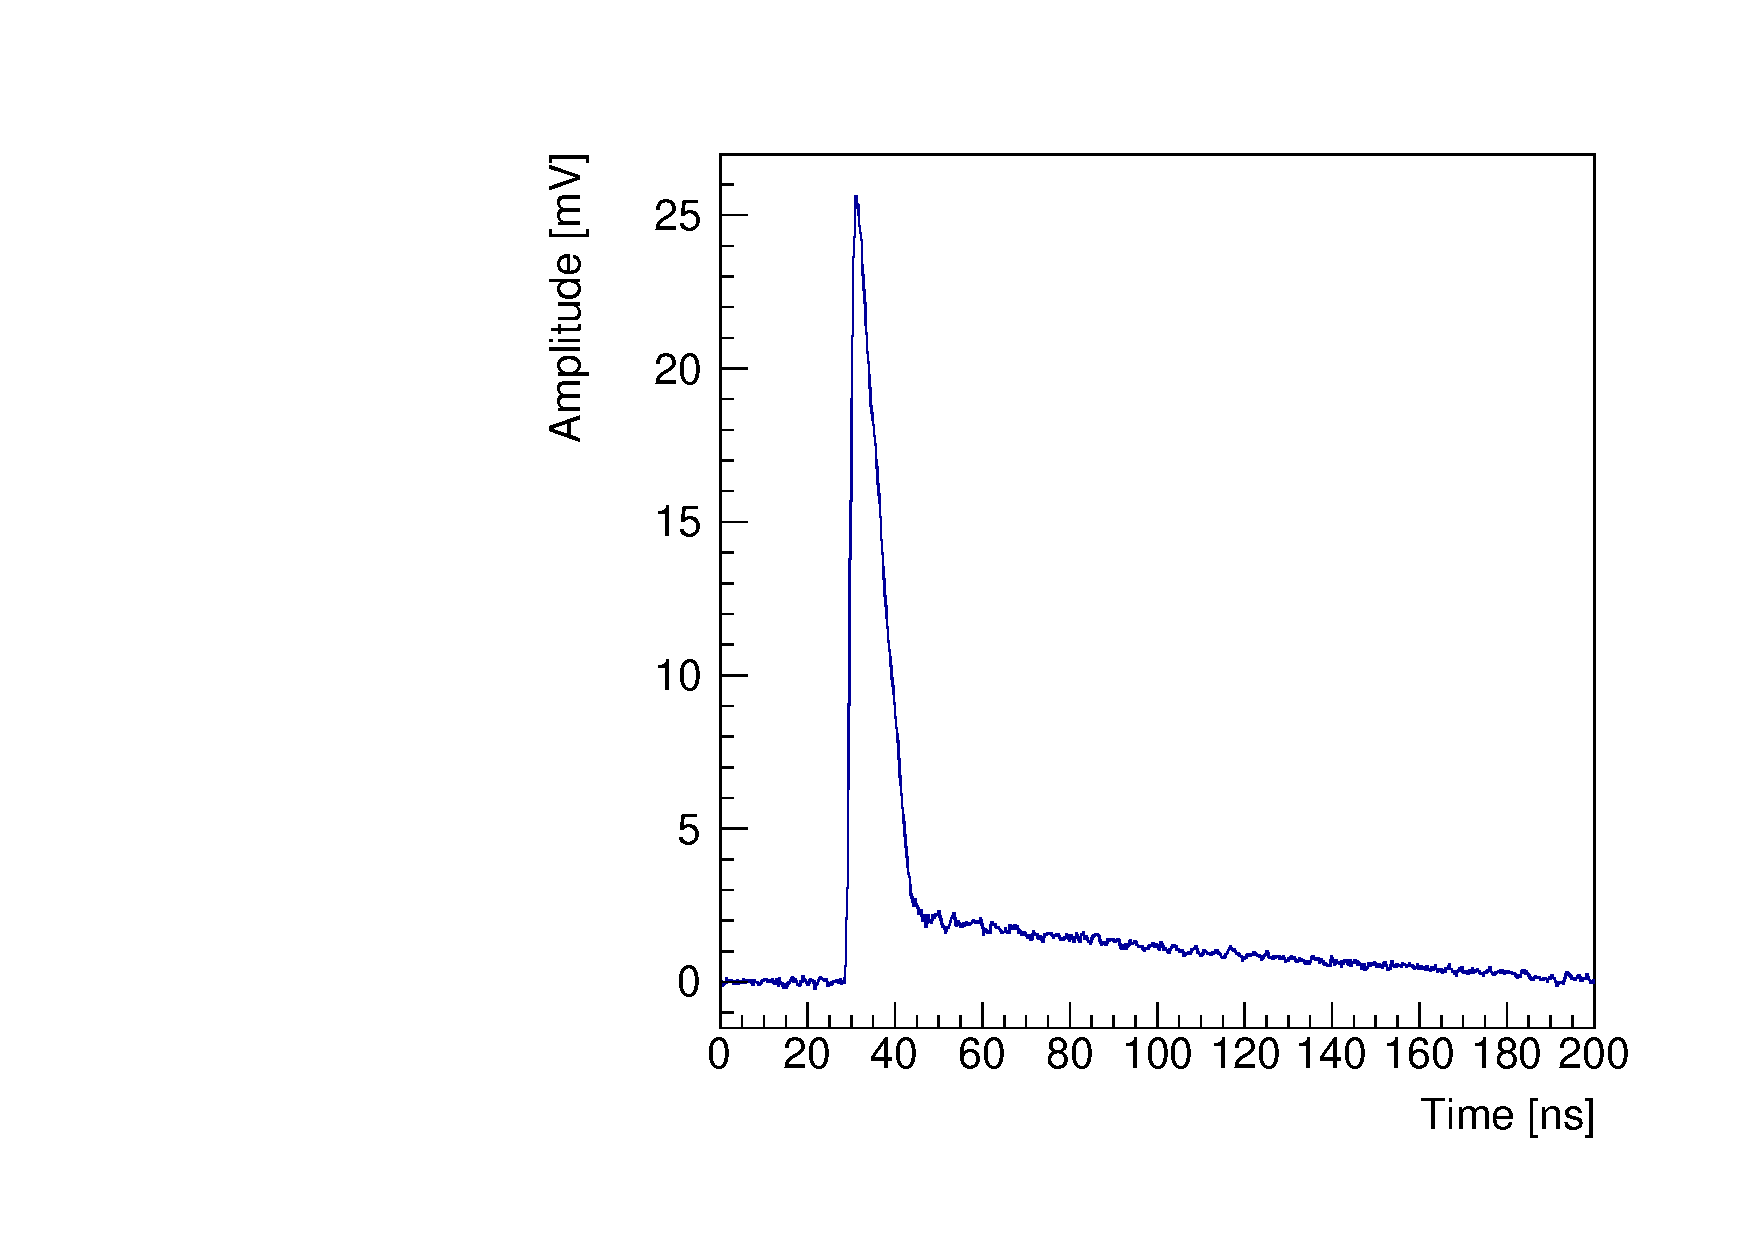
\includegraphics[width=0.49\textwidth]{figures/CdTe_pulse.pdf}
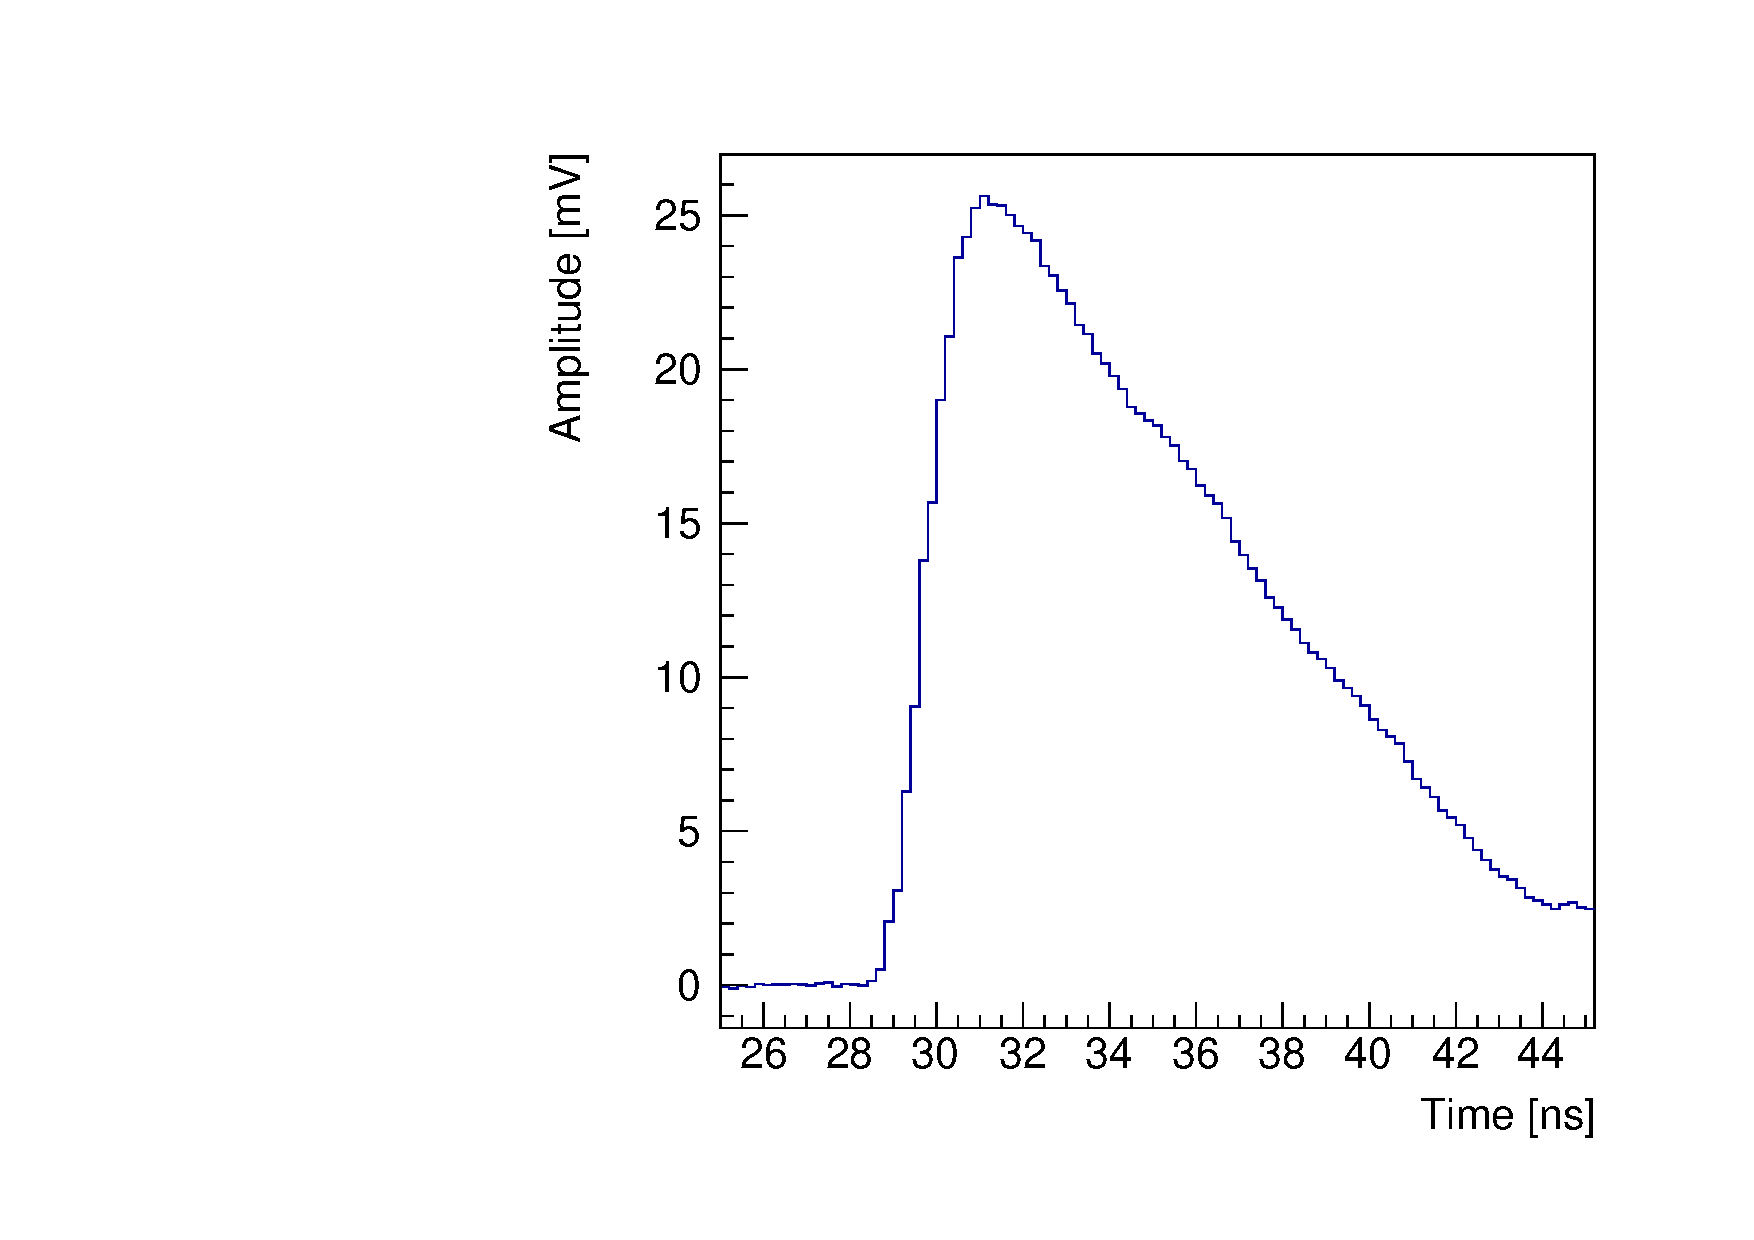
\includegraphics[width=0.49\textwidth]{figures/CdTe_pulseZ.pdf} 
\caption{Examples of signal pulse in the CdTe sensor for electrons with energies of $100$~GeV. 
The signal pulse shown was recorded by the CAEN V1742 digitizer after a $10$~dB 
attenuator and a $36$~dB fast amplifier. Right: Zoom in of the example pulse. } 
\label{fig:Pulses} 
\end{figure} 

The total charge collected in each channel is obtained by computing the integral of the pulse
waveform over the full $200$~ns range recorded by the digitizer. 
The timestamp for each signal is reconstructed by fitting the pulse waveform with
an appropriate functional form. For signal pulses from the MCP-PMTs, used as reference timers, 
we fit a Gaussian function to a $1.5$~ns window around the peak of the pulse and extract the 
timestamp $t_{0}$ as the mean parameter of the Gaussian function. For signal pulses from the
CdTe sensor, we fit a linear function to time sample points between $10\%$ and $60\%$ of the pulse
maximum and the timestamp $t_{1}$ is assigned as the time at which the fitted linear function
rises to $30\%$ of the pulse maximum. More details of the timestamp reconstruction can be
found in reference~\cite{Anderson:2015gha}.


For the measurements performed at the H2 beamline, 
based on the results shown in Figure~\ref{fig:BeamSensorPosition} we select events
for which the incident beam particle lies within a region of size $3$~mm by $3$~mm 
about the center of the sensor. For the measurements performed at the T9 beamline,
the resolution of the wire chamber measurement was insufficient to make this 
requirement. We also require that the 
signal in the reference MCP-PMT detector has an amplitude larger than $25$~mV. 
For data collected at the H2 beamline, the MCP-PMT detector is located behind
the absorbers and can discriminate between electrons that shower in the absorber
material and pions that do not. We require that the signal amplitude in the 
MCP-PMT detector is larger than $500$~mV to select a pure sample of electrons. For
data collected at the T9 beamline, the electron selection is performed using
the LYSO scintillating crystal placed behind the absorber material and the CdTe sensor,
as shown in Figure~\ref{fig:BeamSchematicDiagram}. The electromagnetic shower particles produce
scintillation light in the LYSO crystal and are read out by an MCP-PMT. We require that
the signal amplitude in the MCP-PMT coupled to the LYSO crystal is larger than $800$~mV
to select a sample of pure electrons. Furthermore, as the precision of the beam particle position 
measured by the wire chambers at the T9 beamline is relatively poor, we also require
large signals in the $1$~cm~$\times$~$1$~cm scintillator trigger counter, with
amplitude above $150$~mV, to constrain the beam to a smaller geometric region. 
  
%
%

\section{Calorimetric Measurements} 
\label{sec:calorimetery} 

To obtain a preliminary characterization of the calorimetric performance 
of the CdTe sensors, we measure the total charge collected out of the CdTe 
sensor for various incident electron beam energies. Examples of the 
charge distributions are shown in Figure~\ref{fig:ChargeDistribution}
for $2$~GeV and $200$~GeV electrons. For electrons with energy between 
$2$~GeV and $7$~GeV, the sensor was placed after $2$ radiation lengths 
of absorber material, and for electrons with energy above $50$~GeV, the 
sensor was placed after $6$ radiation lengths of absorber material.

%Fig: Charge distributions (noise, showers, MIP?)
\begin{figure}[htbp] 
\centering
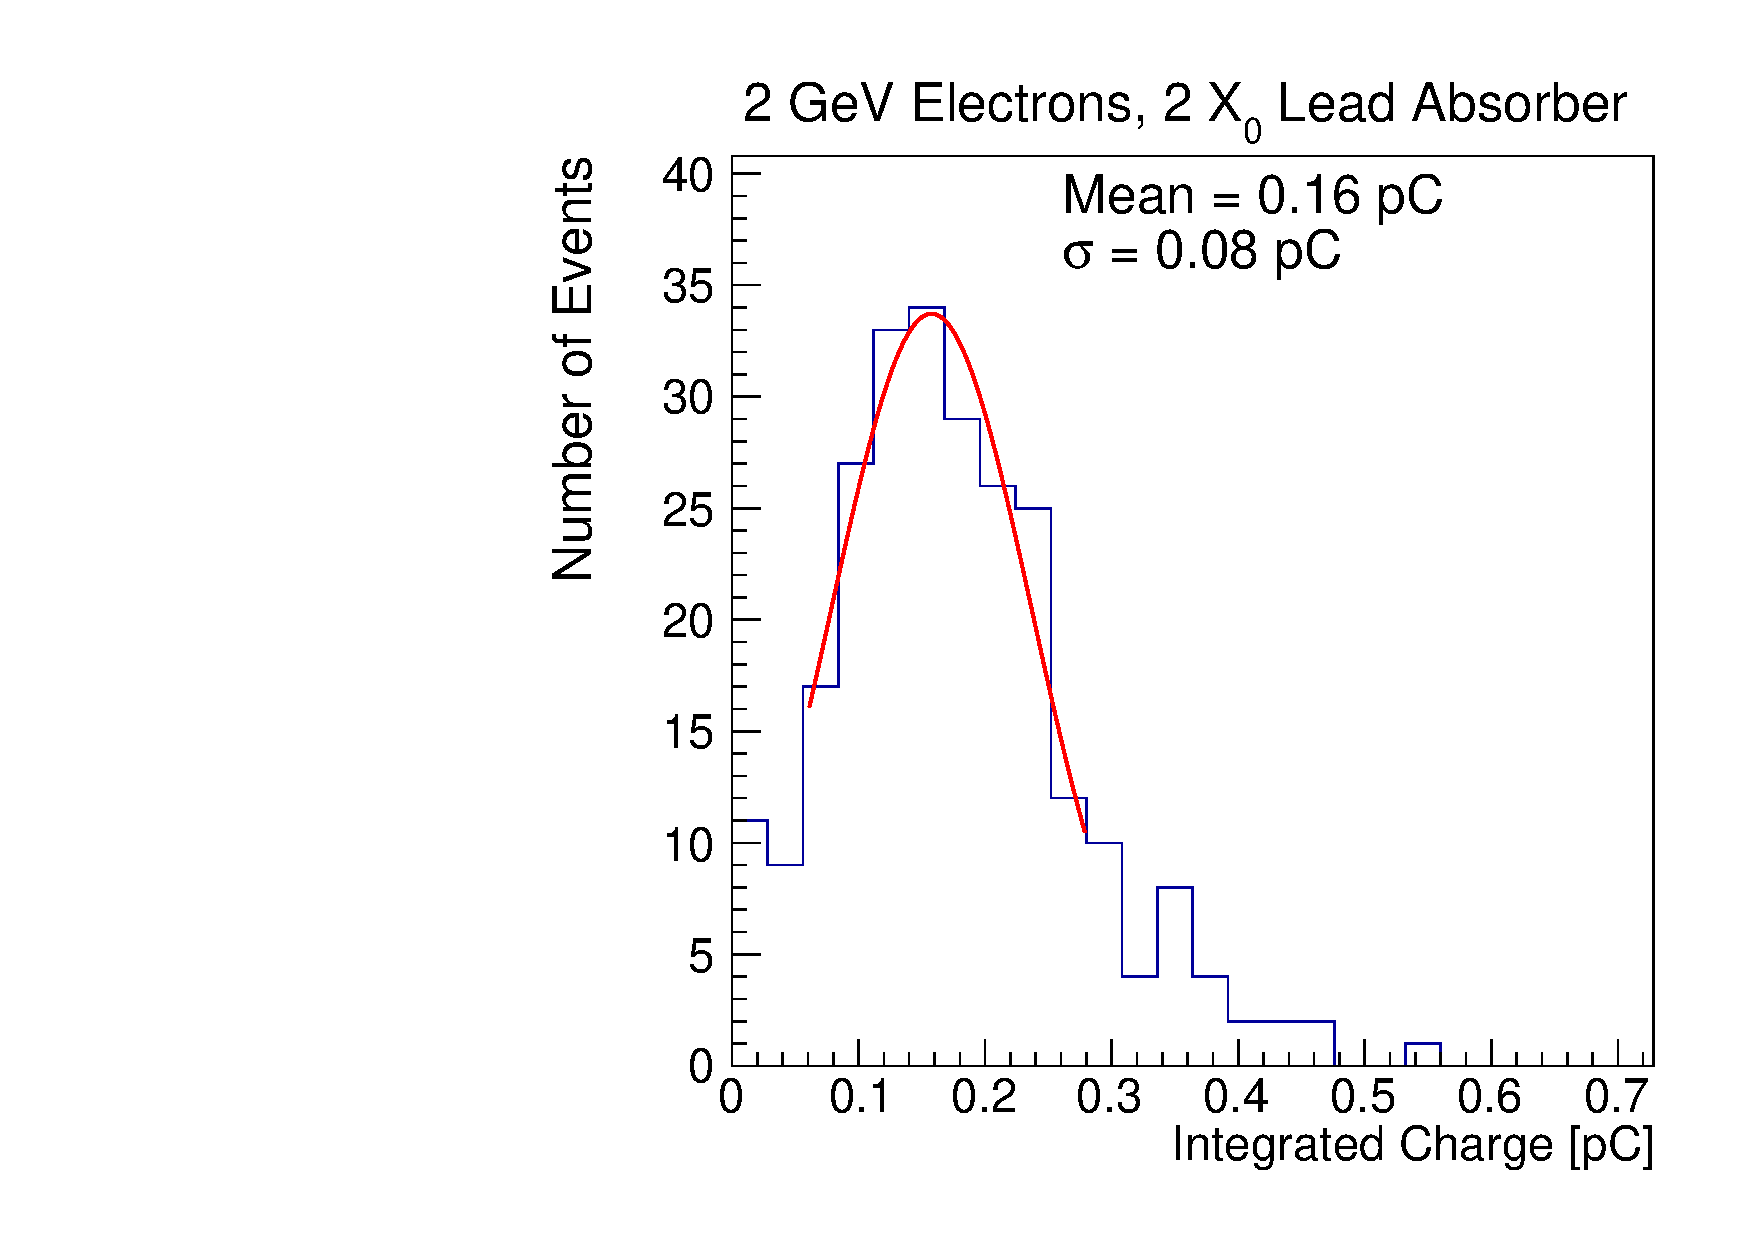
\includegraphics[width=0.49\textwidth]{figures/2GeV_charge.pdf} 
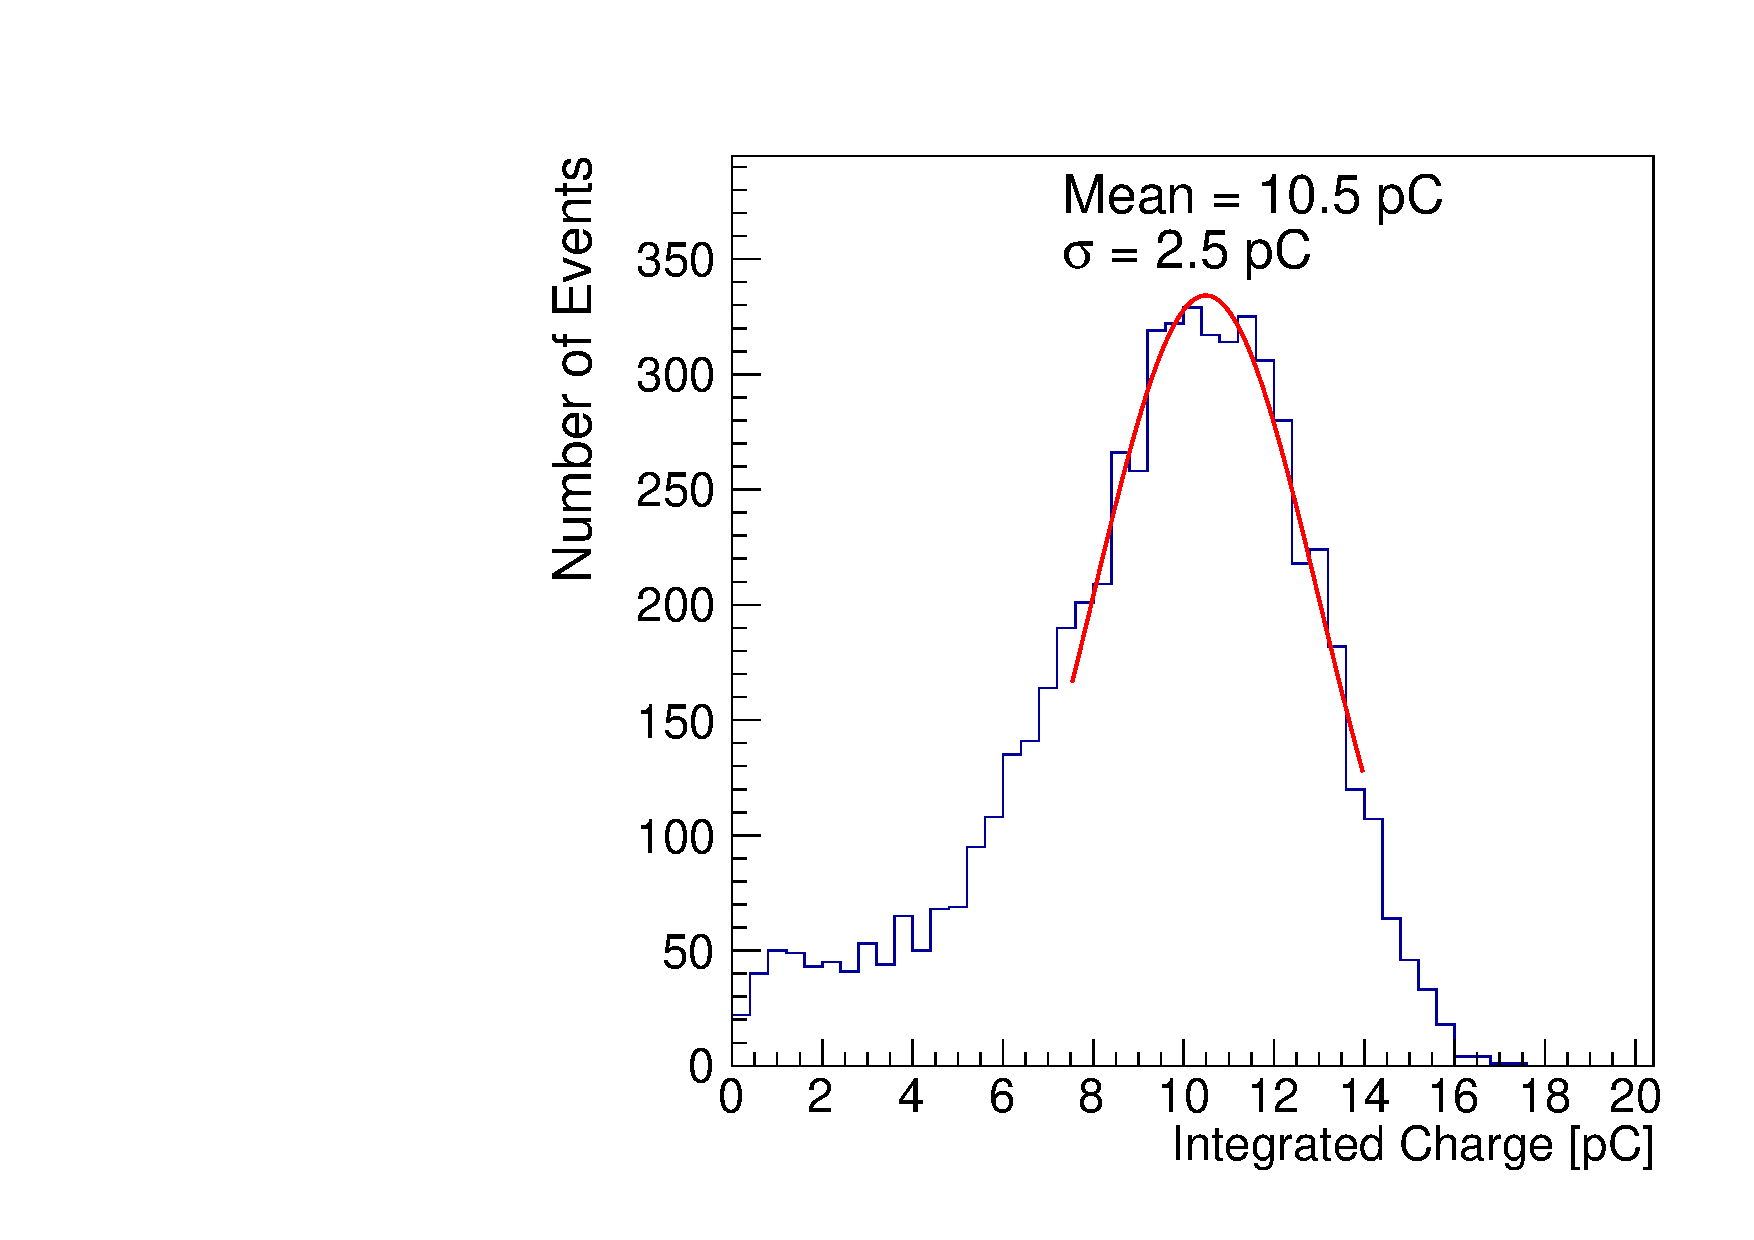
\includegraphics[width=0.49\textwidth]{figures/200GeV_charge.pdf} 
\caption{Distribution of total charge collected in the CdTe sensor for a $2$~GeV
electron after $2$~$\mathrm{X}_{0}$ of lead absorber (left) and a 200~GeV
electron after $6$~$\mathrm{X}_{0}$ of tungsten absorber (right). } 
\label{fig:ChargeDistribution} 
\end{figure} 

We plot the mean collected charge as a function of the incident beam energy
in Figure~\ref{fig:ChargeVsEnergy} and observe that the signal size scales
up with increasing beam energy. The resolution is measured as the width
parameter of a Gaussian fit to the charge distribution and is shown by the green
error bars. The measured resolution ranges from
about $50\%$ for electrons in the range of a few GeV to 
about $30\%$ for electrons above $50$~GeV. 
These resolution measurements are encouraging given that they are performed
using only a single layer sample covering a relatively small transverse
geometric area. In future studies, we intend to complete measurements of the
longitudinal shower profile and to instrument a larger transverse 
area to improve the transverse shower containment. 

%Fig: Collected Charge vs Beam Energy
\begin{figure}[htbp] 
\centering
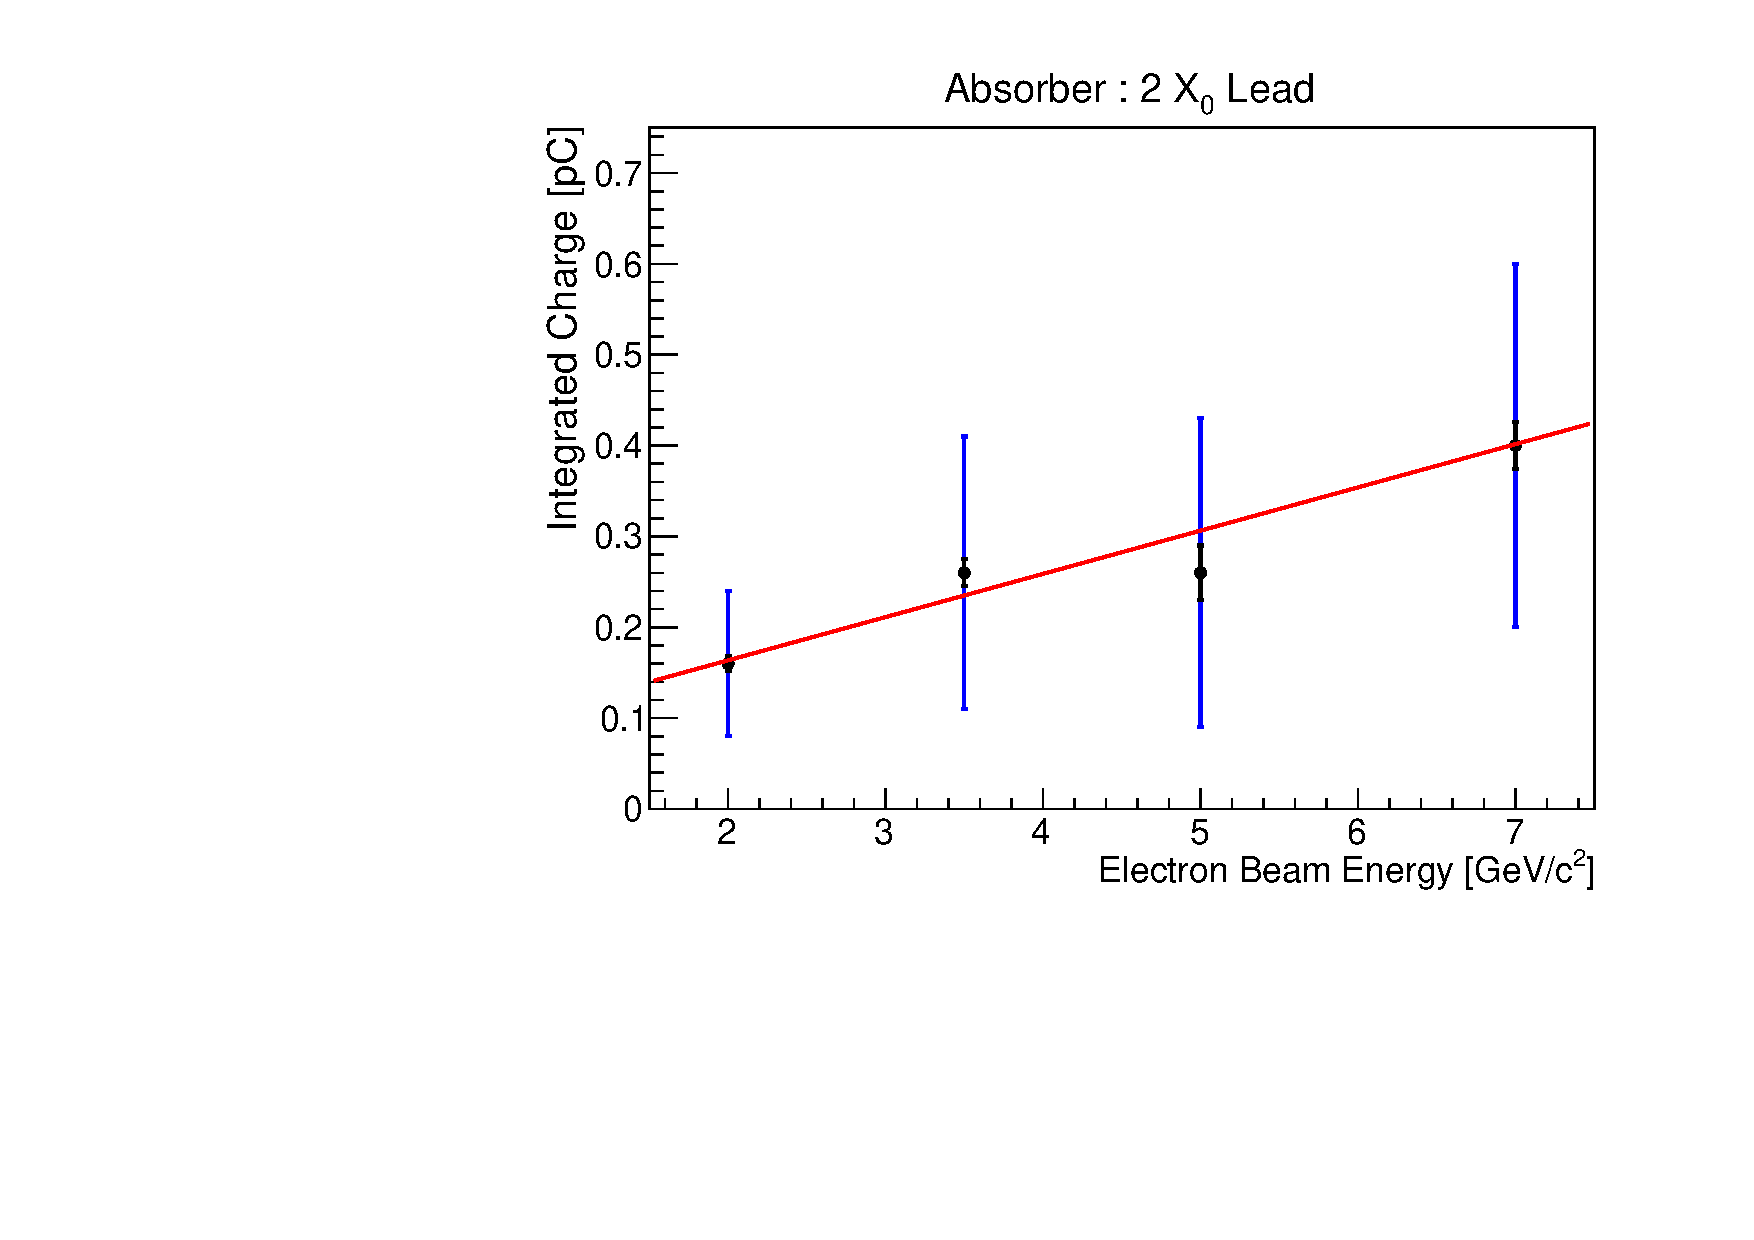
\includegraphics[width=0.49\textwidth]{figures/ChargeVsEnergyAt2X0.pdf} 
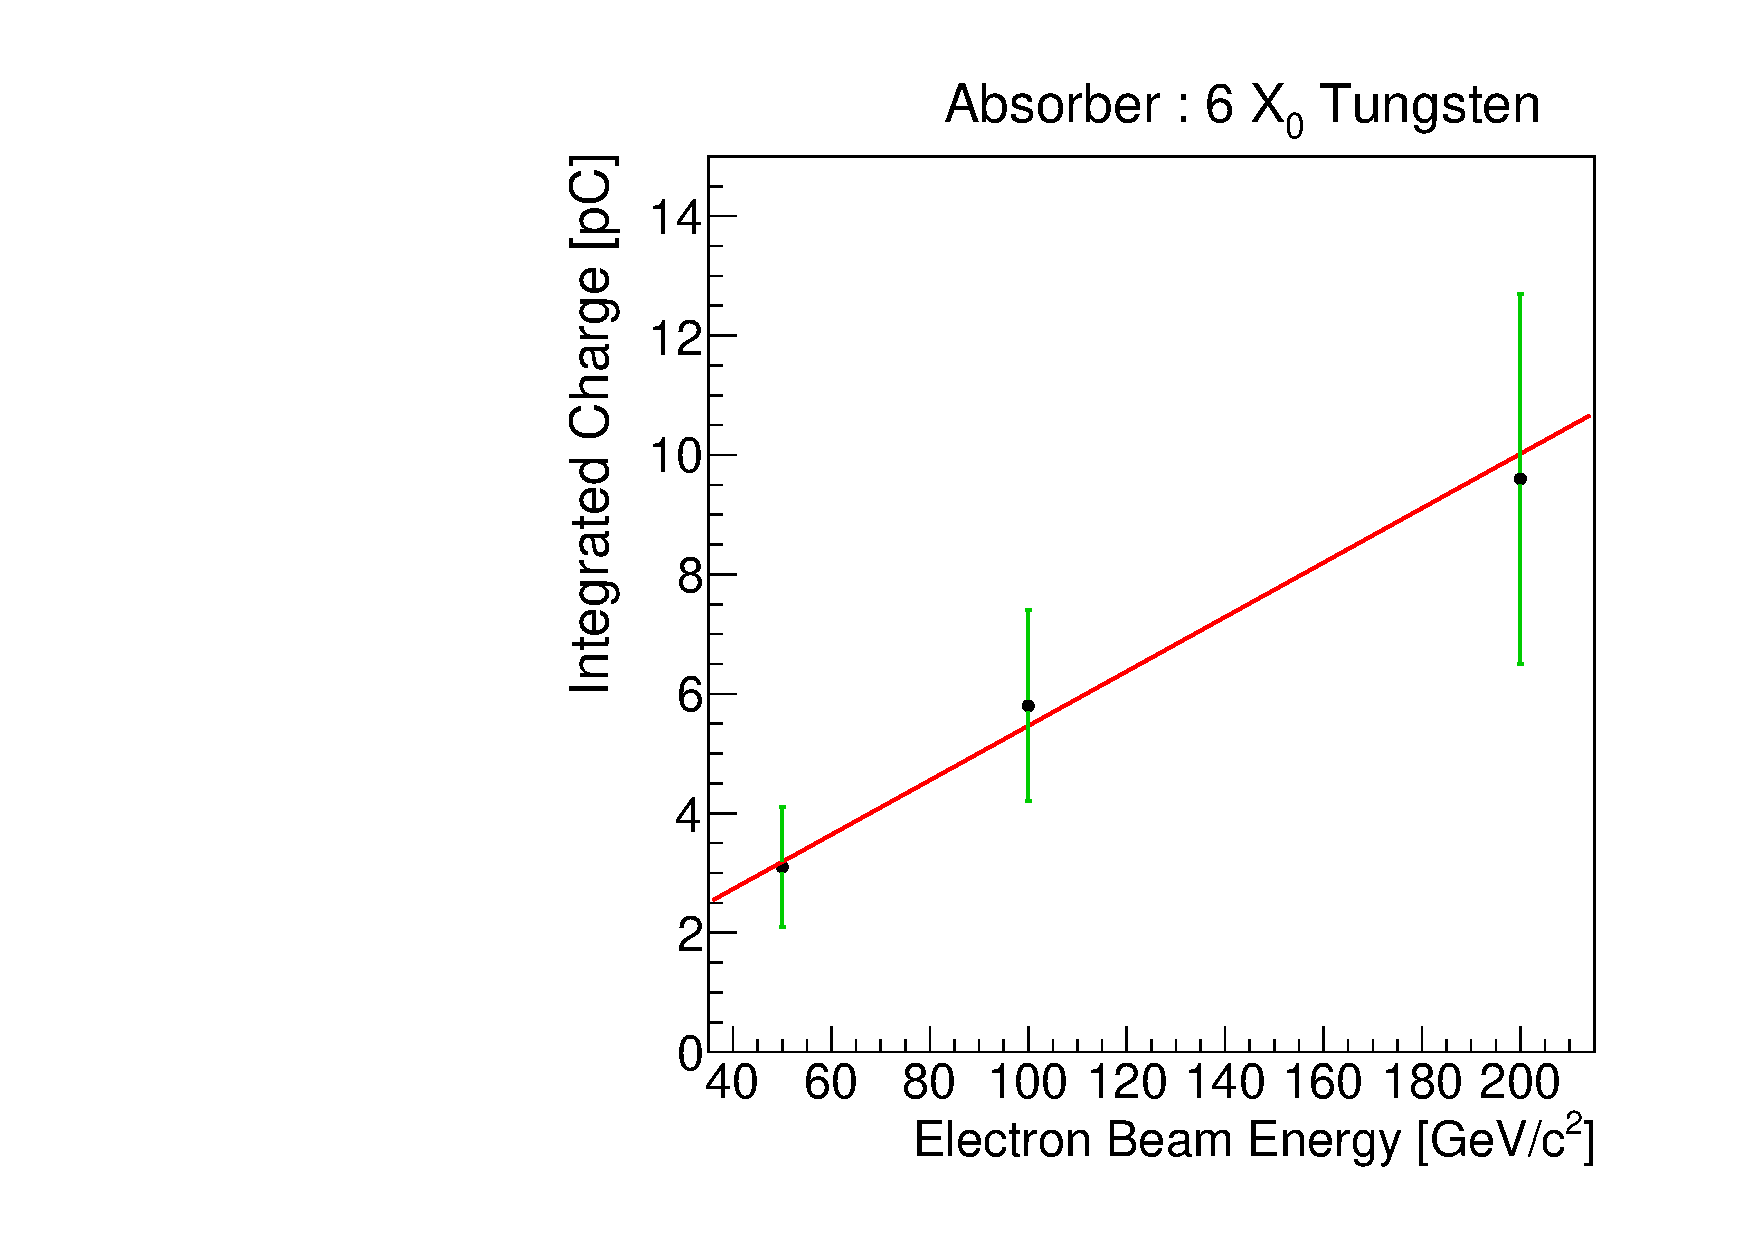
\includegraphics[width=0.49\textwidth]{figures/ChargeVsEnergyAt6X0.pdf} 
\caption{ The mean charge collected in the CdTe sensor is plotted as a function
of the electron beam energy. Left: Measurements performed at the T9 beamline
with $2$~$\mathrm{X}_{0}$ of lead absorber placed directly in front of the 
CeTe sensor. Right: Measurements performed at the H2 beamline
with $6$~$\mathrm{X}_{0}$ of tungsten absorber placed directly in front of the 
CeTe sensor. The blue error bars show the uncertainty on the mean integrated charge,
while the green error bars show the measured resolution. The red line is a 
linear fit to each set of measured data. } 
\label{fig:ChargeVsEnergy} 
\end{figure} 


  
%
%

\section{Timing Measurements} 
\label{sec:timing} 

We characterize the timing performance of the CdTe sensor by measuring the time-stamps
relative to the MCP-PMT device used as a reference timer. An example of the distribution 
of the time-stamp measurement for $100$~GeV electrons after $6$~$\mathrm{X}_{0}$ of 
tungsten absorber is shown in Figure~\ref{fig:DeltaT}. We extract the time measurement
resolution from this distribution as the width parameter of a Gaussian fit.
In Figure~\ref{fig:TimeResolutionVsEnergy} we show the measured time resolution as a function of the
beam energy. For beam energies between $2$~GeV and $50$~GeV, the time resolution 
improves with increasing signal size as expected based on the increasing signal-to-noise ratio.
However, above $100$~GeV, the time resolution no longer improves with 
increasing signal size, which points towards some systematic limitation. 
We study a number of such factors in Section~\ref{sec:systematicLimitations} below.

%Figure: example DeltaT plot
\begin{figure}[htbp] 
\centering
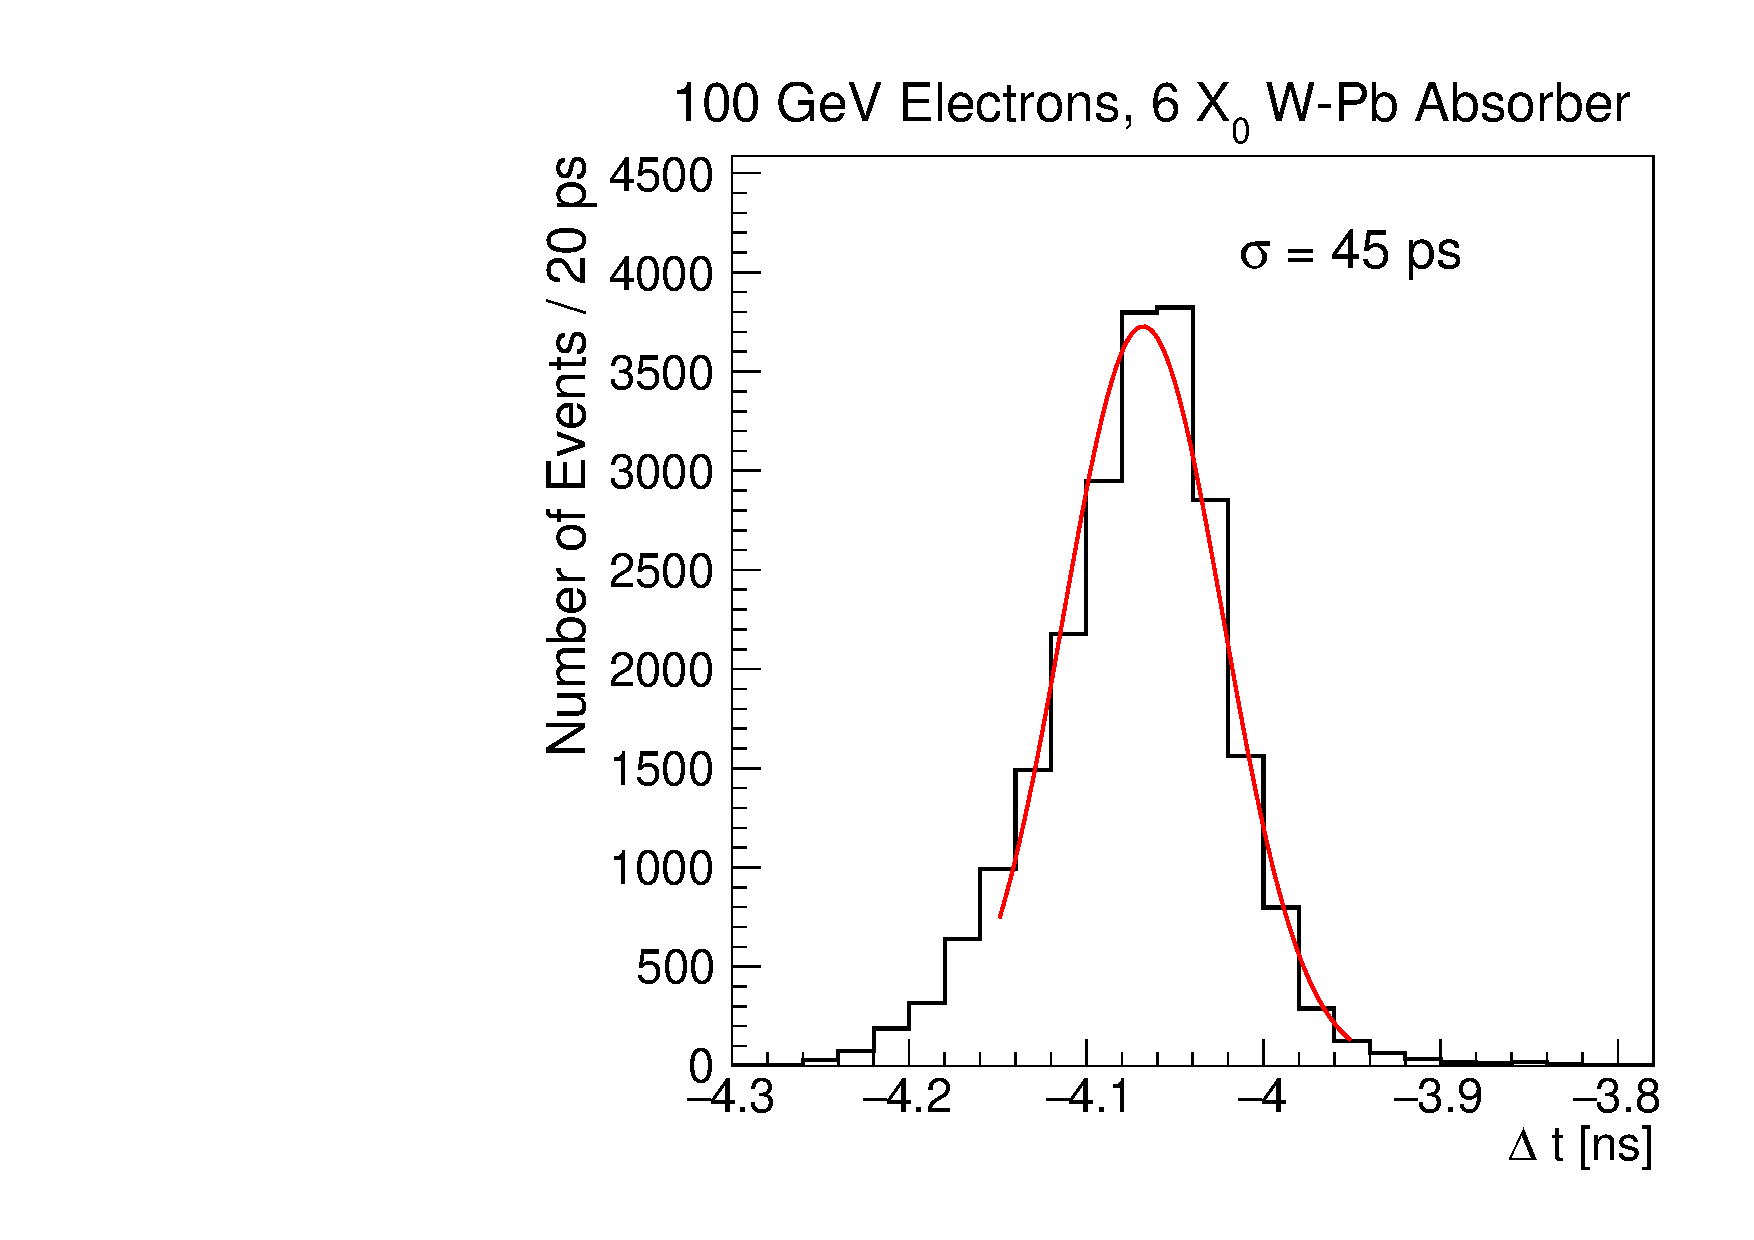
\includegraphics[width=0.49\textwidth]{figures/100GeV_deltaT.pdf} 
\caption{Distribution of the time-stamp measurement in the CdTe sensor for a $100$~GeV
electron after $6$~$\mathrm{X}_{0}$ of tungsten and lead absorber. } 
\label{fig:DeltaT} 
\end{figure} 


%Figure: Time resolution vs beam energy
\begin{figure}[htbp] 
\centering
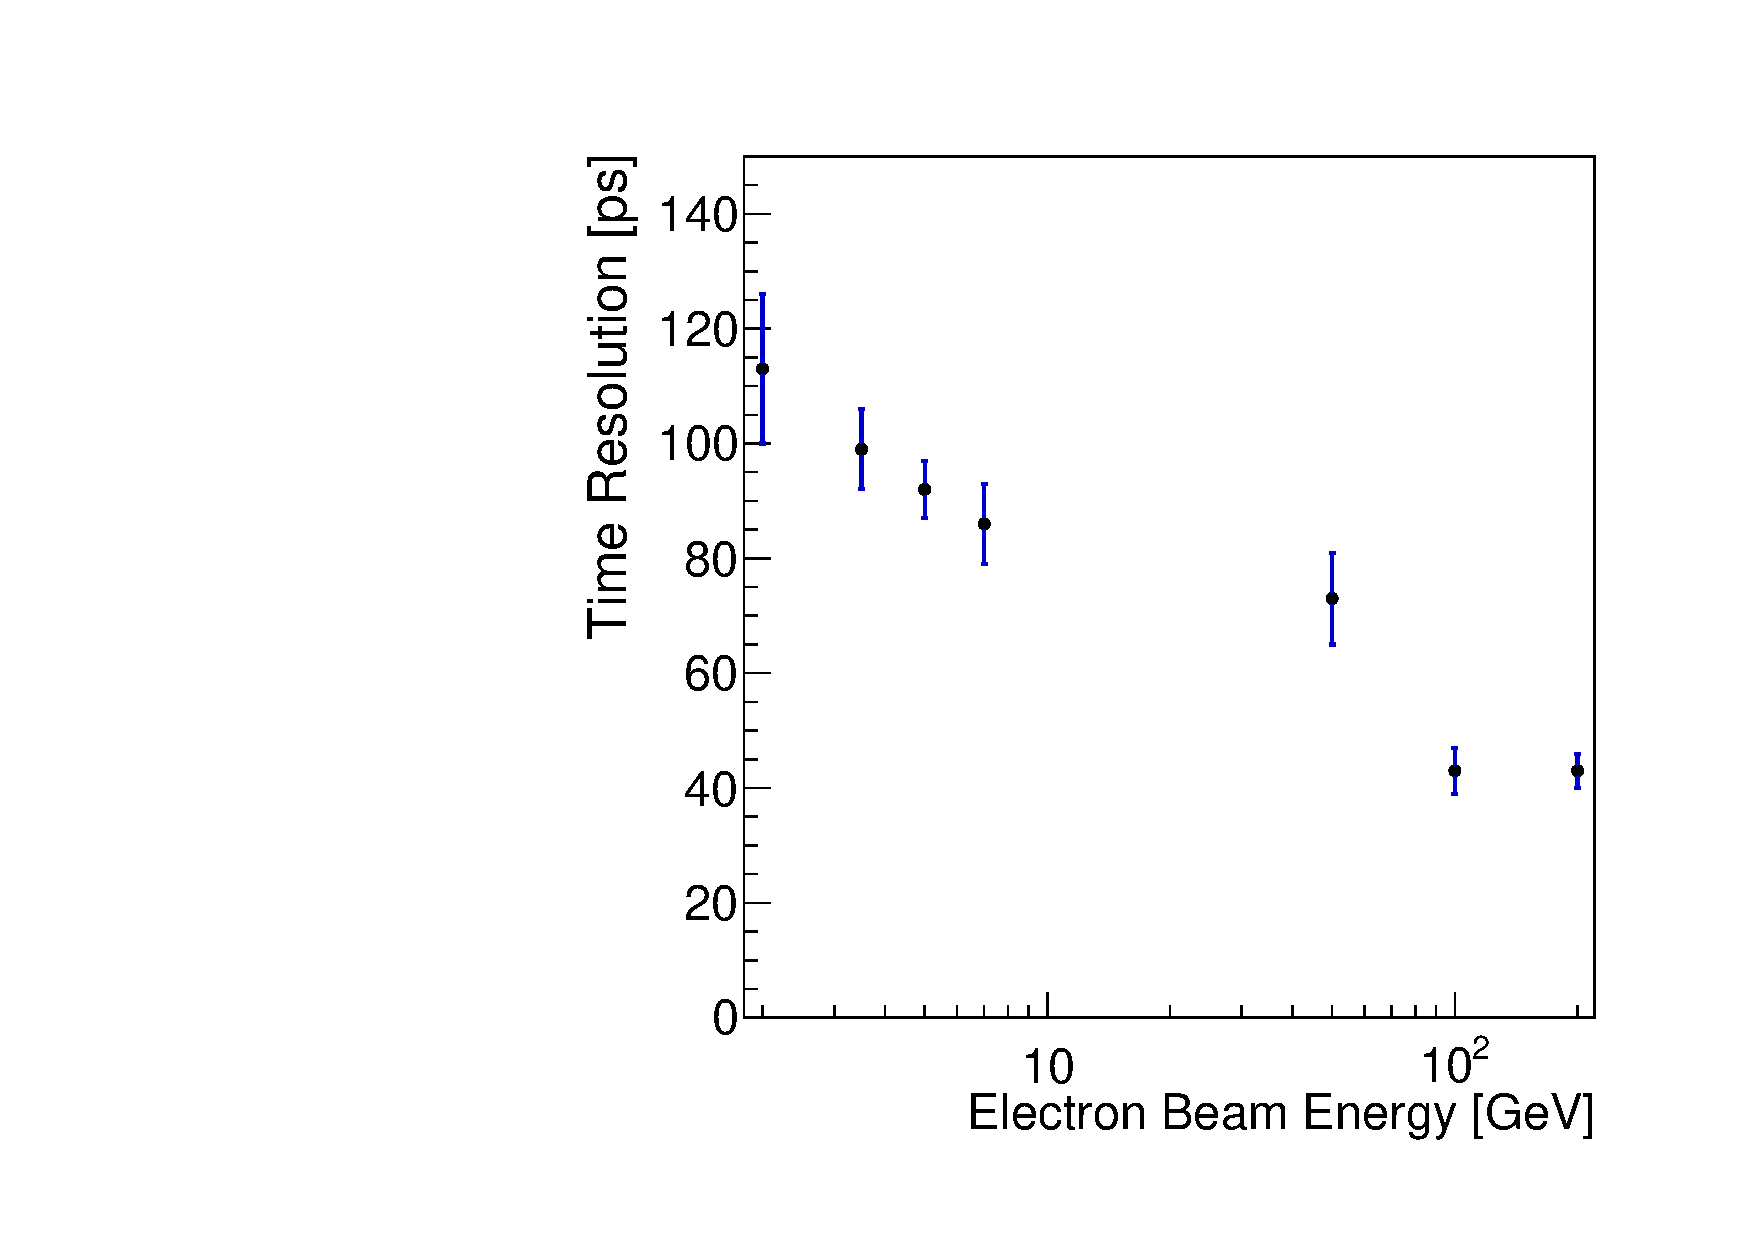
\includegraphics[width=0.49\textwidth]{figures/TimeResolutionVsEnergy.pdf} 
\caption{ The measured time resolution of the CdTe sensor is plotted as a function
of the electron beam energy. } 
\label{fig:TimeResolutionVsEnergy} 
\end{figure} 


To further characterize the timing performance of the CdTe signals, we measure the
rise-time, defined as the time for the signal to rise from $10\%$ to $90\%$ of its maximum
amplitude, for various electron beam energies. The distribution of rise-time for
$100$~GeV electrons and the measured rise-time as a function of the beam energy
are shown on the left and right of Figure~\ref{fig:riseTime} respectively. 
We observe a rise-time of around $1.3$~ns that does not vary significantly
with the beam energy.


%Figure: riseTime vs energy
\begin{figure}[htbp] 
\centering
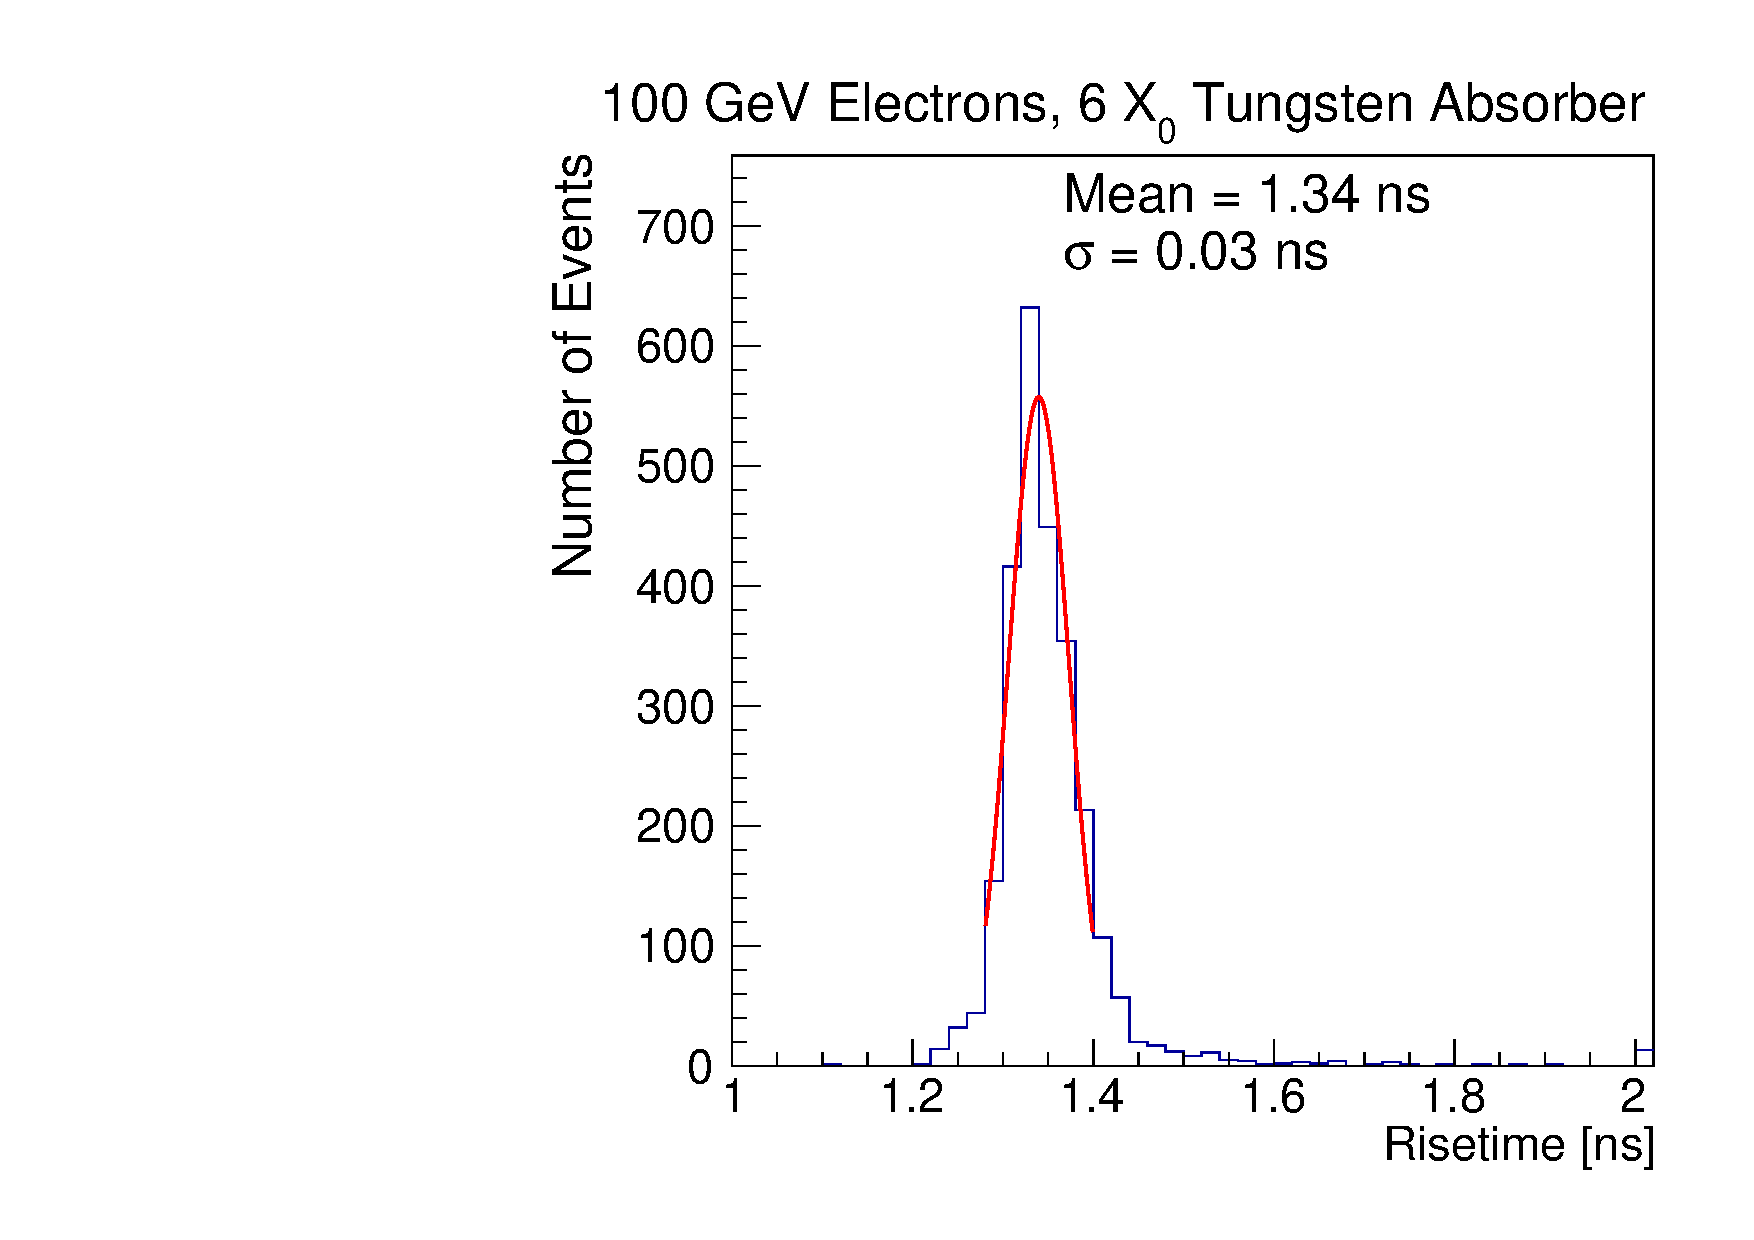
\includegraphics[width=0.49\textwidth]{figures/100GeV_risetime.pdf} 
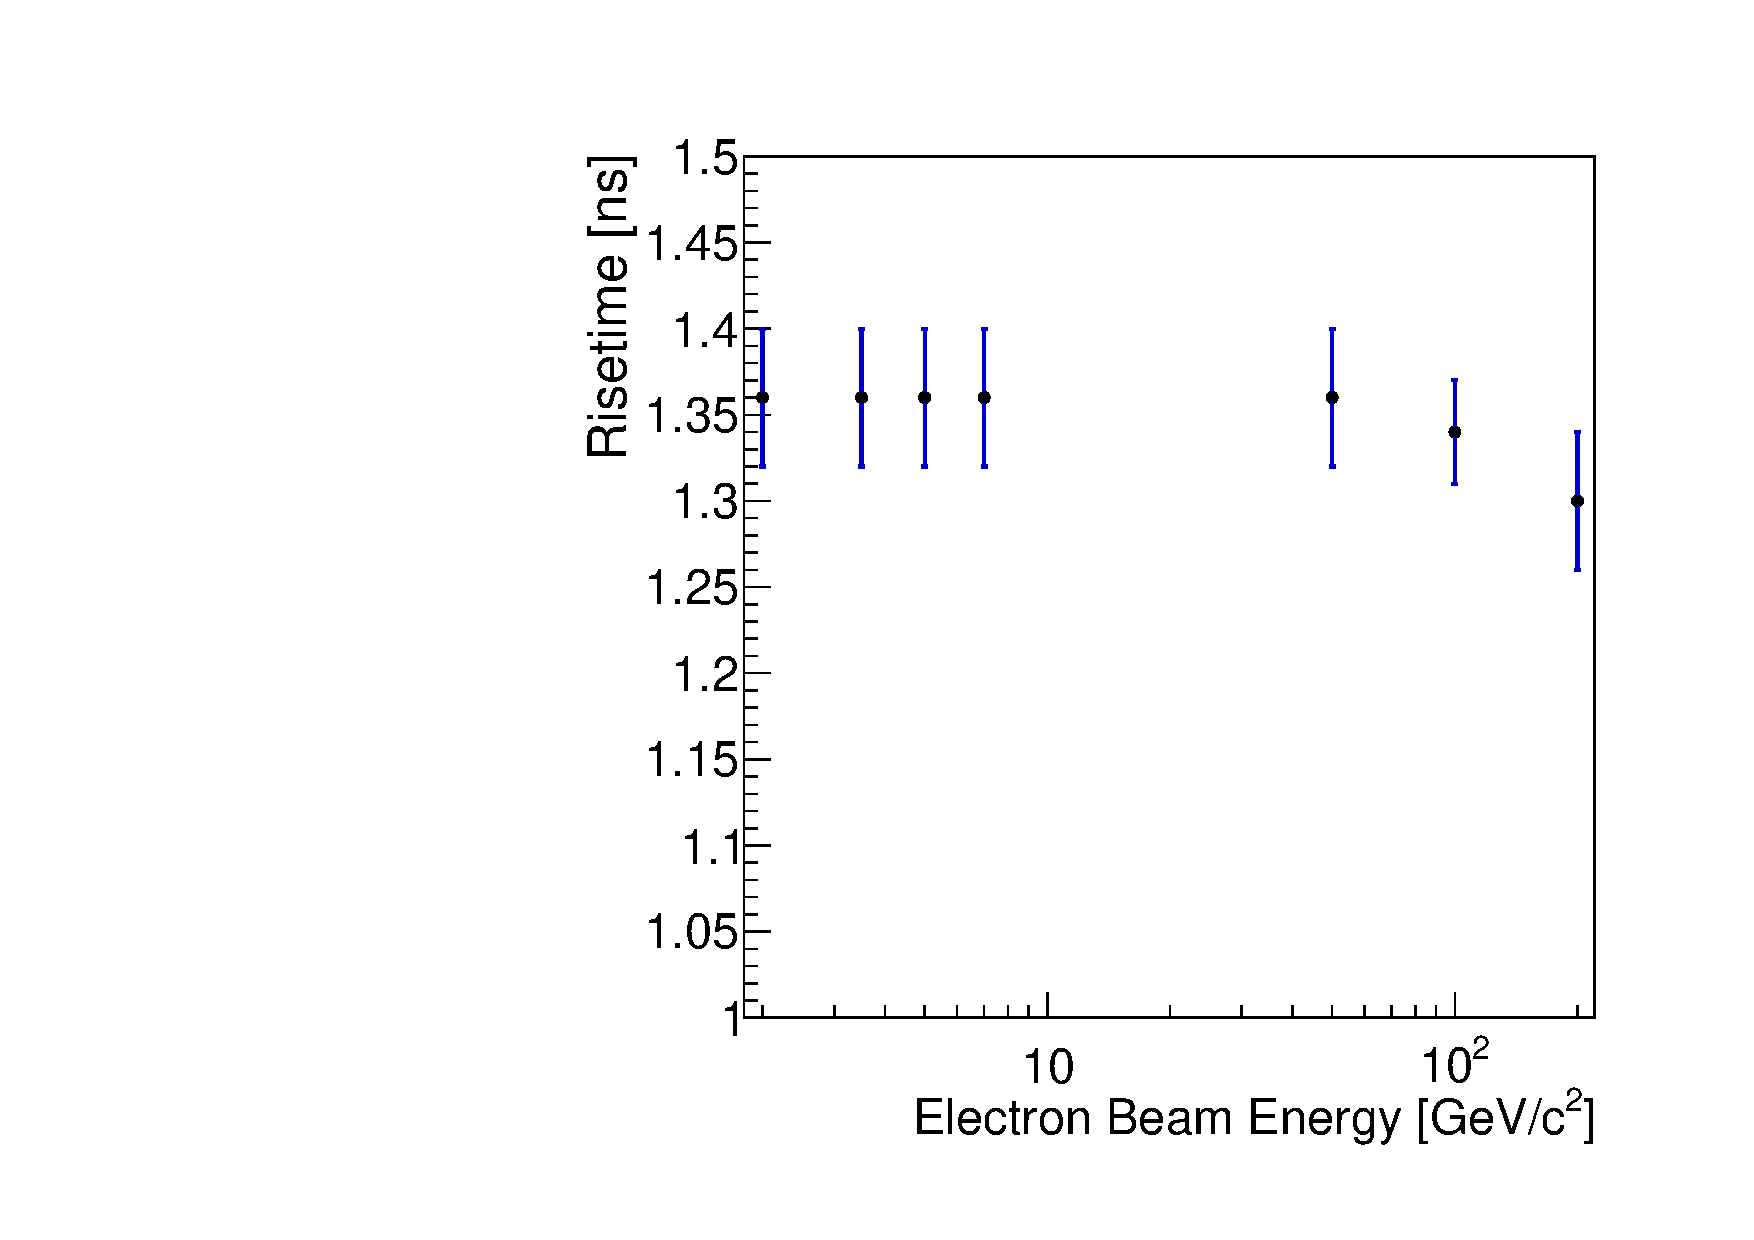
\includegraphics[width=0.49\textwidth]{figures/RisetimeVsEnergy.pdf} 
\caption{ Left: Distribution of rise-time of the CdTe signal for $100$~GeV electrons. 
Right: Rise-time of the CdTe signal is plotted as a function of the incident beam energy. 
The uncertainty is extracted from the width of the fitted gaussian to the rise-time 
distribution. 
} 
\label{fig:riseTime} 
\end{figure} 



\subsection{Studies of Systematic Limitations on Time Resolution}
\label{sec:systematicLimitations}

One of the major systematic effects that have been observed in past
timing studies~\cite{Anderson:2015gha,Ronzhin201552,MCPShowerMaxPaper} is the dependence 
of the time measurement on the amplitude of the signal. On the left of 
Figure~\ref{fig:DeltaTVsAmplitude}, we show the dependence of the time-stamp measurement 
on the amplitude of the signal, and observe a mild dependence on amplitude, which we correct for
in subsequent figures.
On the right of Figure~\ref{fig:DeltaTVsAmplitude}, we show the measured time resolution
as a function of the signal amplitude and we observe a clear improvement
in the resolution with increasing signal amplitudes up to $0.5$~V.
In this region, the impact of the signal-to-noise ratio is still 
the dominant factor for the time resolution.

%Figure: DeltaT vs Amplitude
\begin{figure}[htbp] 
\centering
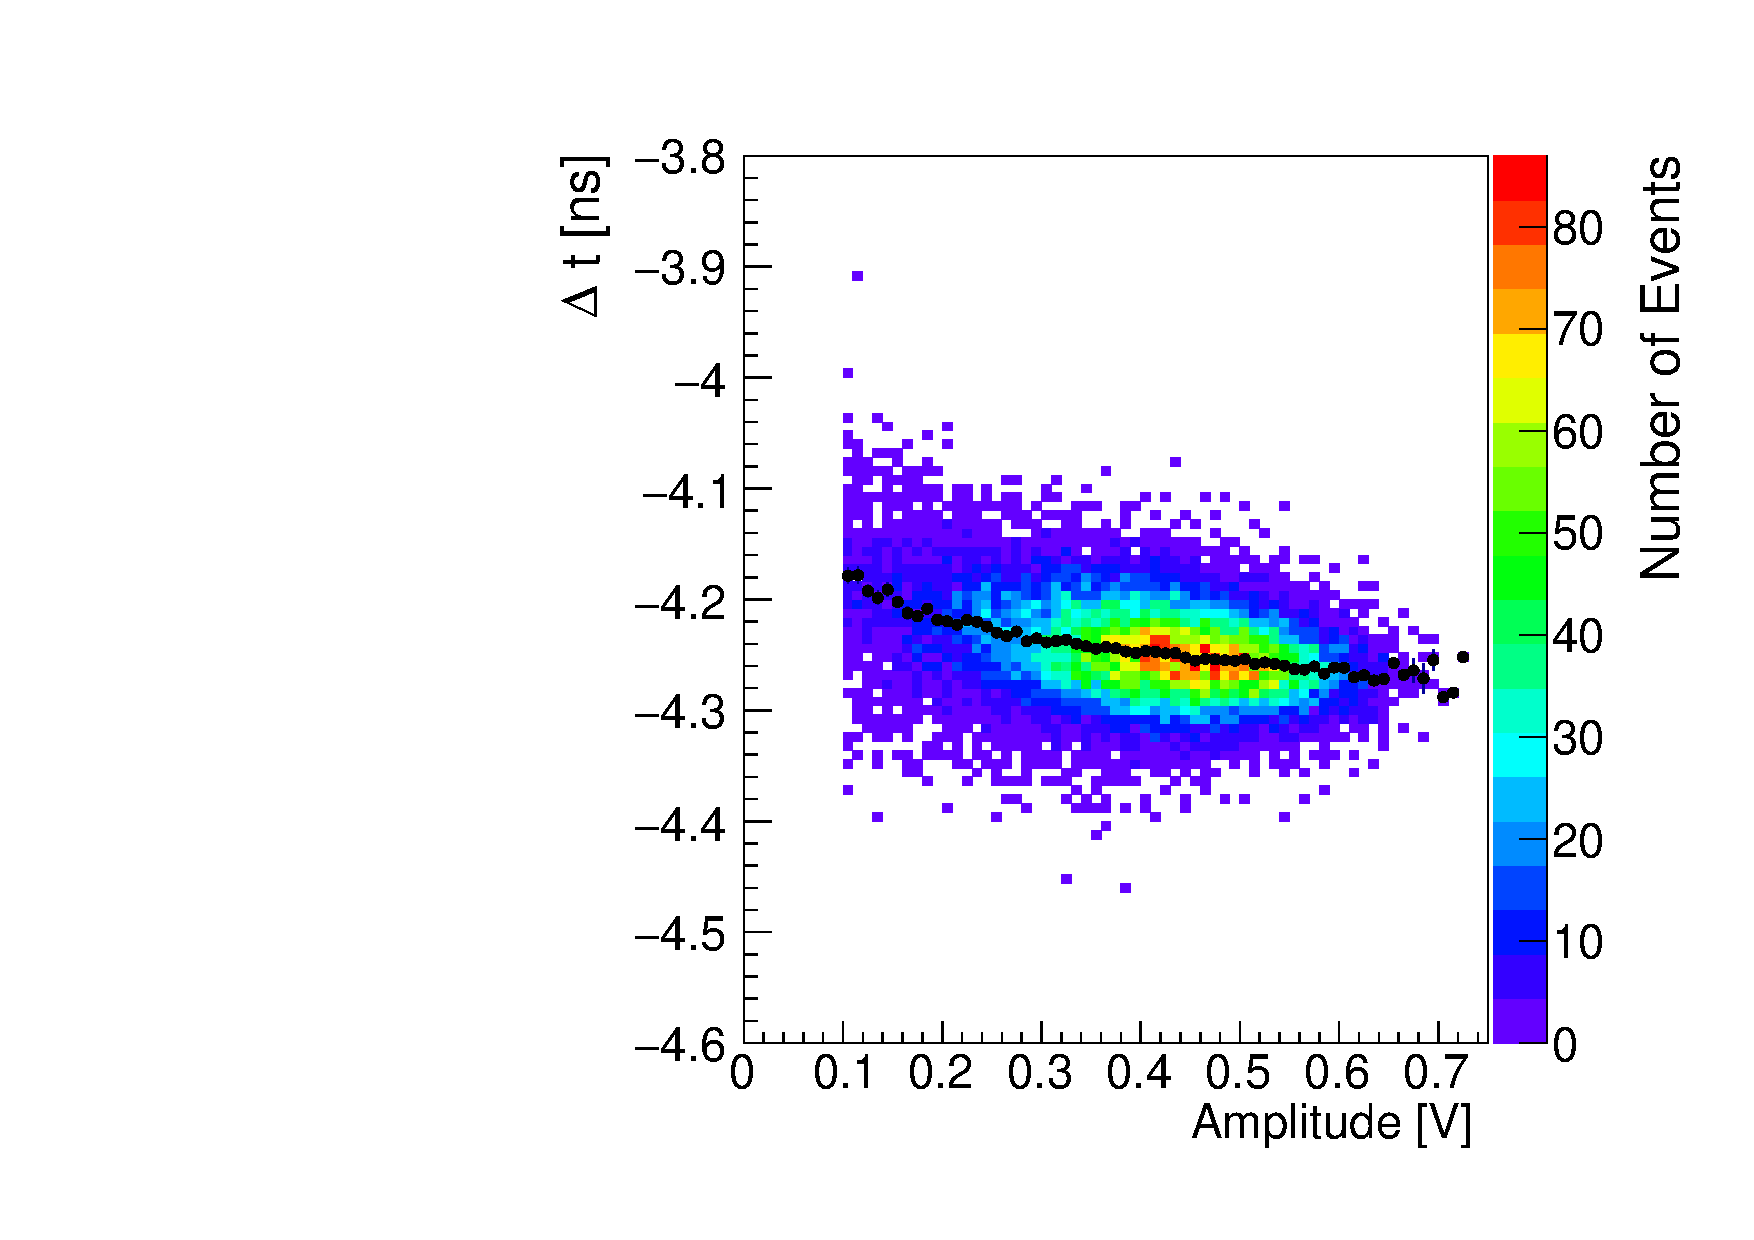
\includegraphics[width=0.49\textwidth]{figures/100GeV_deltaTVsAmp.pdf} 
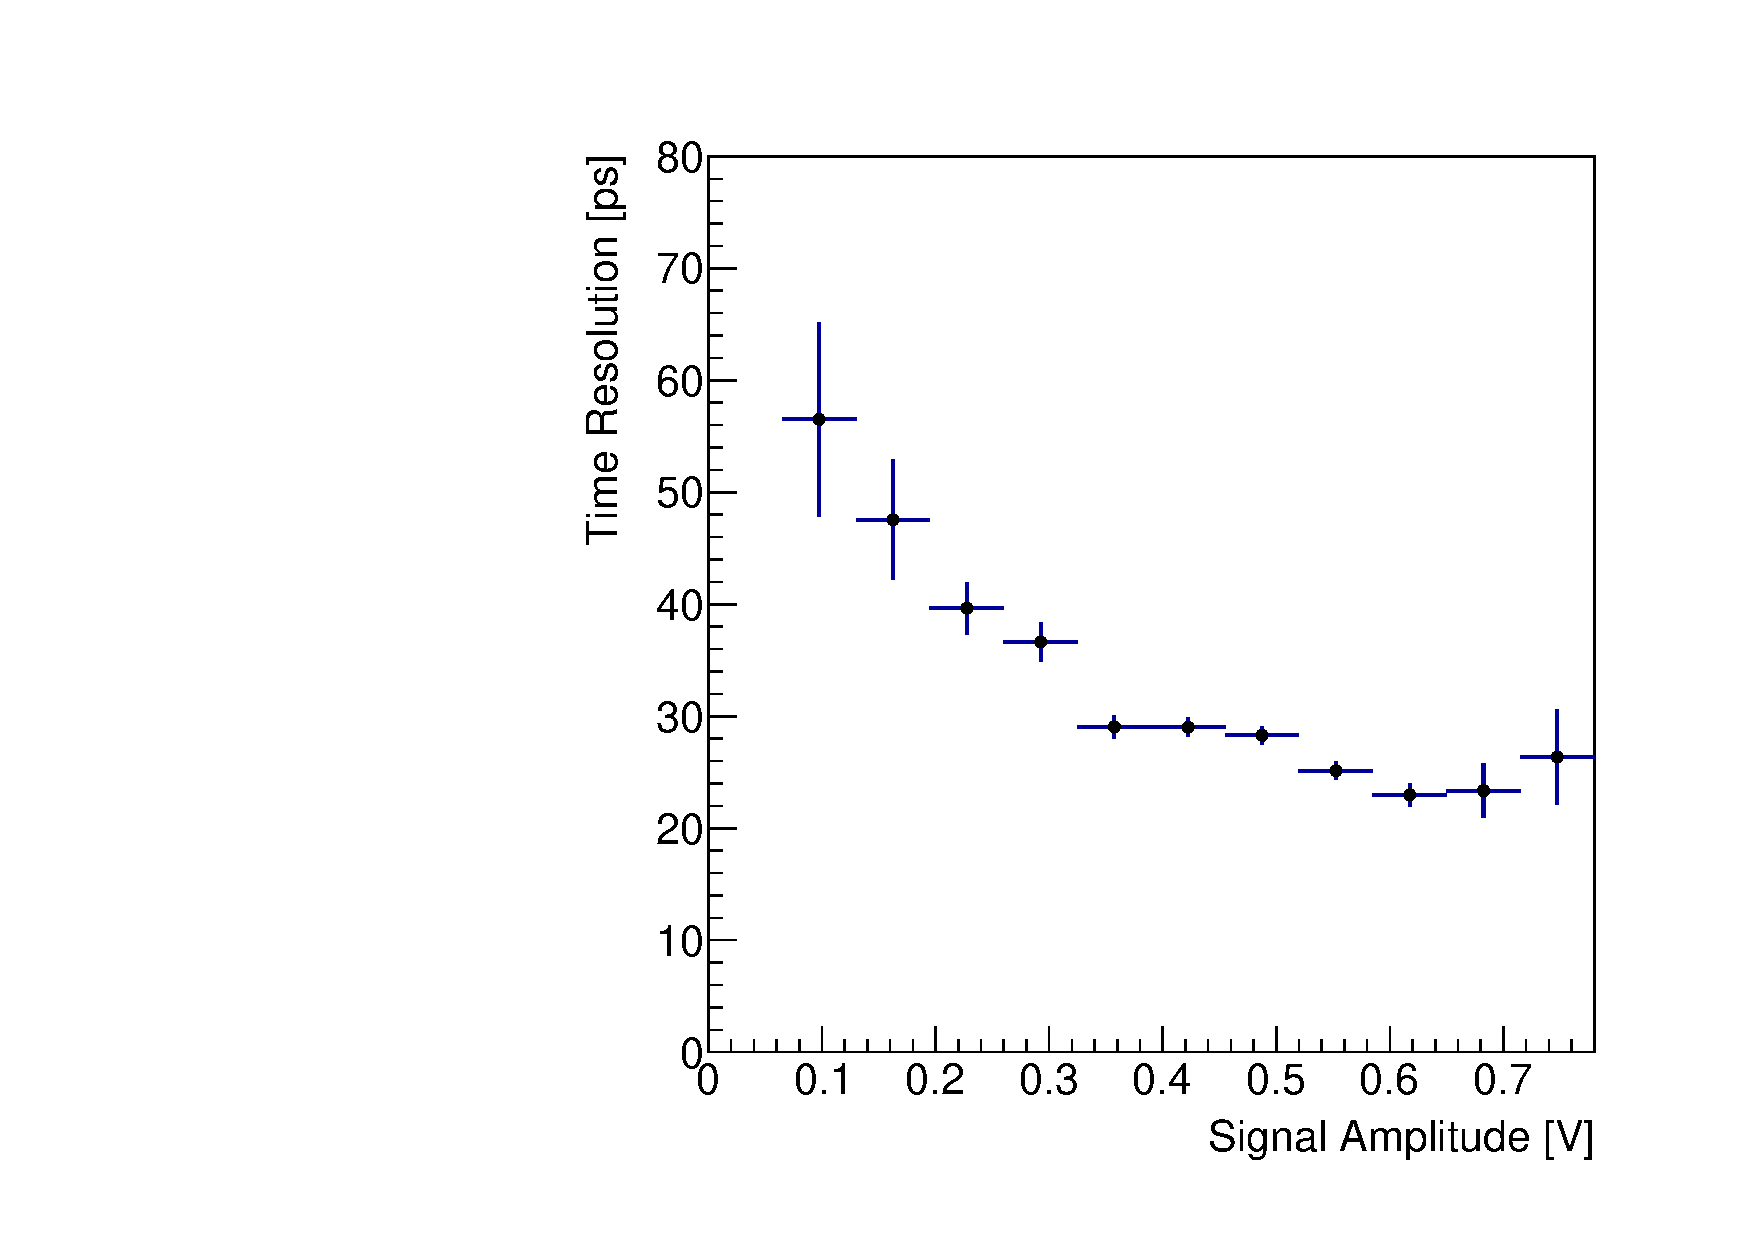
\includegraphics[width=0.49\textwidth]{figures/TimeResolutionVsAmplitude.pdf} 
\caption{ Left: The distribution of the signal amplitude in the CdTe sensor and 
the time measured in the CdTe sensor relative to the Photek reference detector
is shown in the color scale. This data is from a $100$~GeV electron beam after $6$~$X_0$ absorber.
The mean value of the time measured in the CdTe sensor 
as a function of the signal amplitude is shown in the black points. 
Right: The time resolution is measured as a function of the signal amplitude after correction
for amplitude non-linearity. } 
\label{fig:DeltaTVsAmplitude} 
\end{figure} 


We also study the dependence of the time-stamp measurement as a function of the geometric
position of the incident beam particle as measured by the wire chambers in 
Figure~\ref{fig:DeltaTVsBeamXY}. A relatively large and linear dependence is observed, 
and this position non-uniformity of the time response adds significantly to the 
time resolution (about $37$~ps). Performing a correction for this non-uniformity improves
the time resolution from $45$~ps to $25$~ps for events with $100$~GeV electrons.
The distribution of time-stamps after correcting for the geometric position is shown
in Figure~\ref{fig:DeltaTCorr}. The measured time resolution, after correction for
the position non-uniformity, has a mild dependence on the beam particle position 
and is shown in Figure~\ref{fig:TimeResolutionVsBeamXY}. Combining the time resolution
dependence on the horizontal and vertical beam positions, we measure the time resolution
as a function of the planar distance between the beam position and the location of the 
back wire bond on the CdTe sensor, and observe a more clear dependence shown in 
Figure~\ref{fig:TimeResolutionVsR}. More detailed studies are necessary
to derive a better understanding of this effect. It will be crucial for any precision timing device
using planar semi-conductor sensors to study the uniformity of the response to achieve an optimal performance.
%
%Figure: DeltaT vs Beam Location
\begin{figure}[htbp] 
\centering
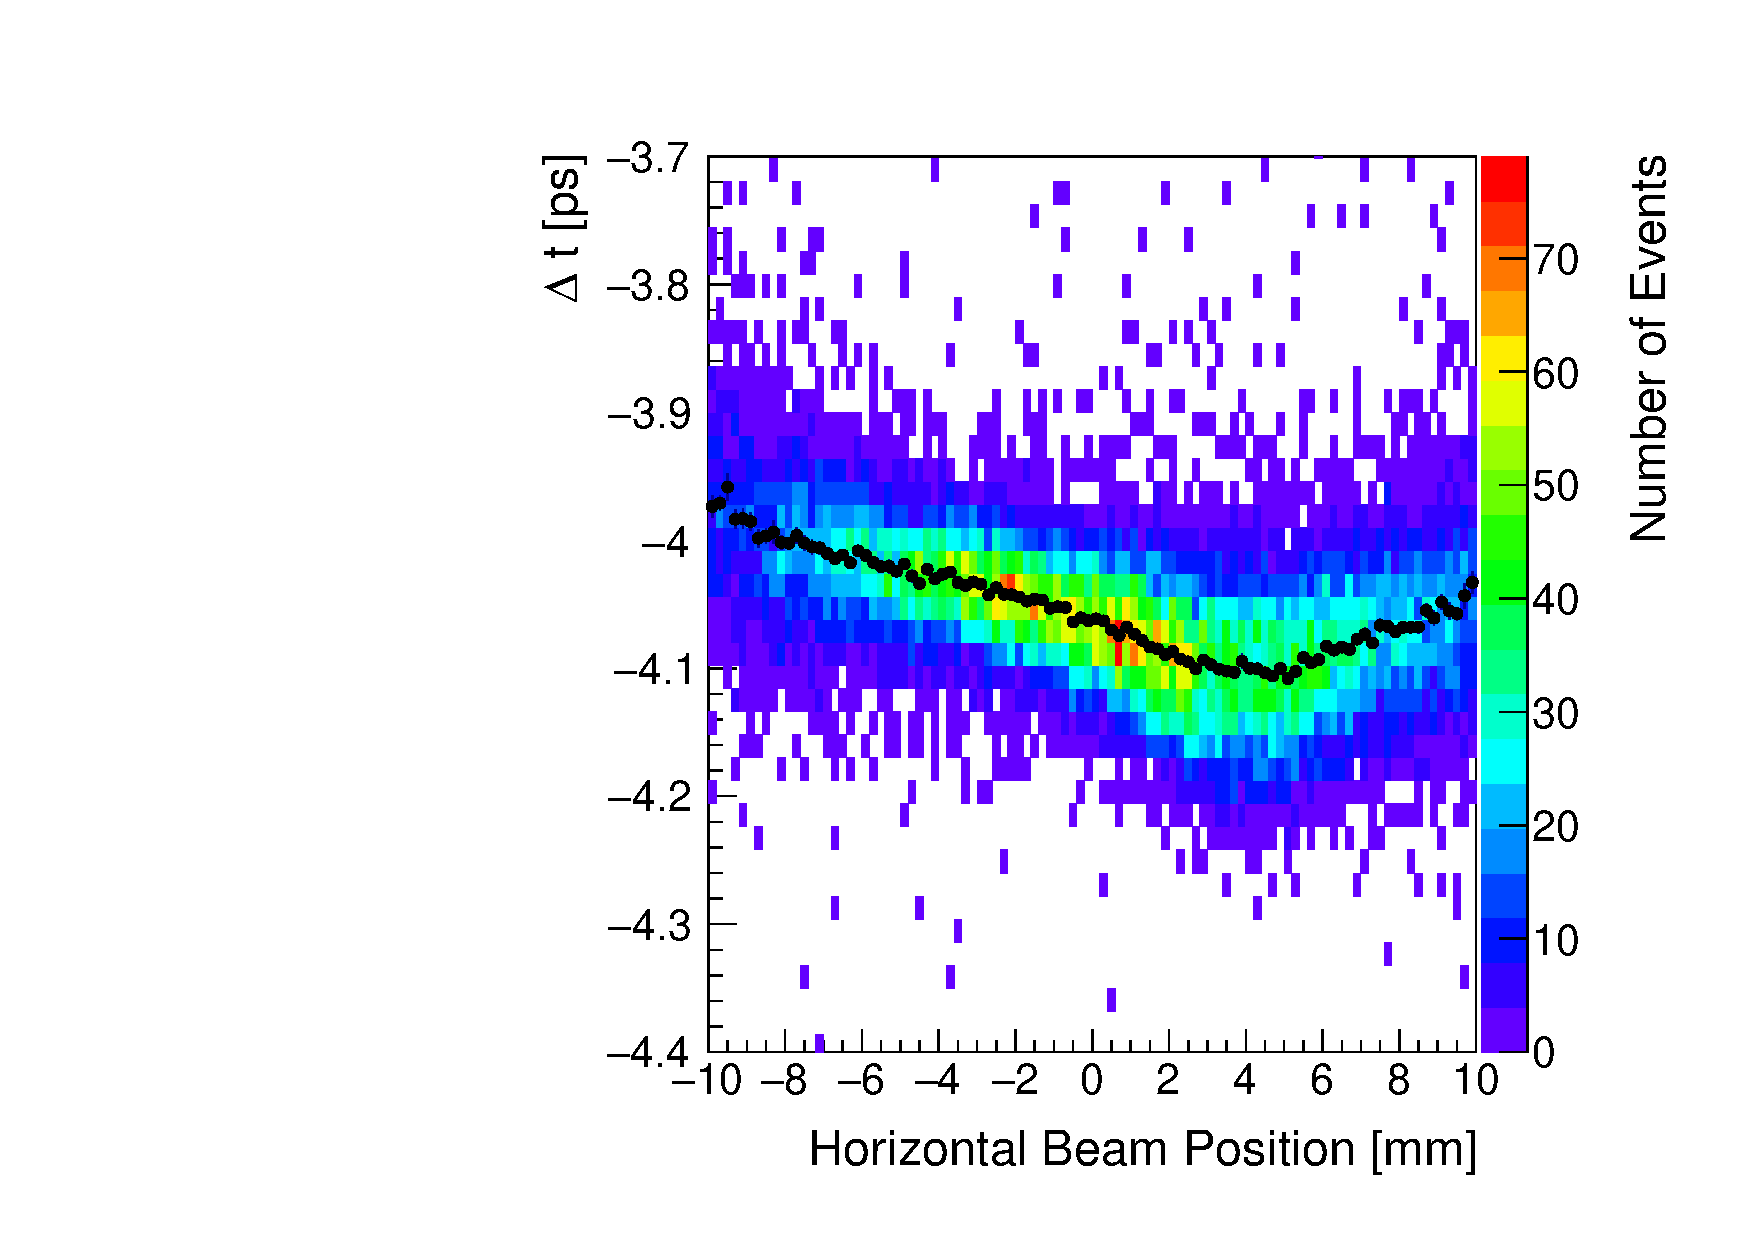
\includegraphics[width=0.49\textwidth]{figures/DeltaTVsHorizontalPosition.pdf} 
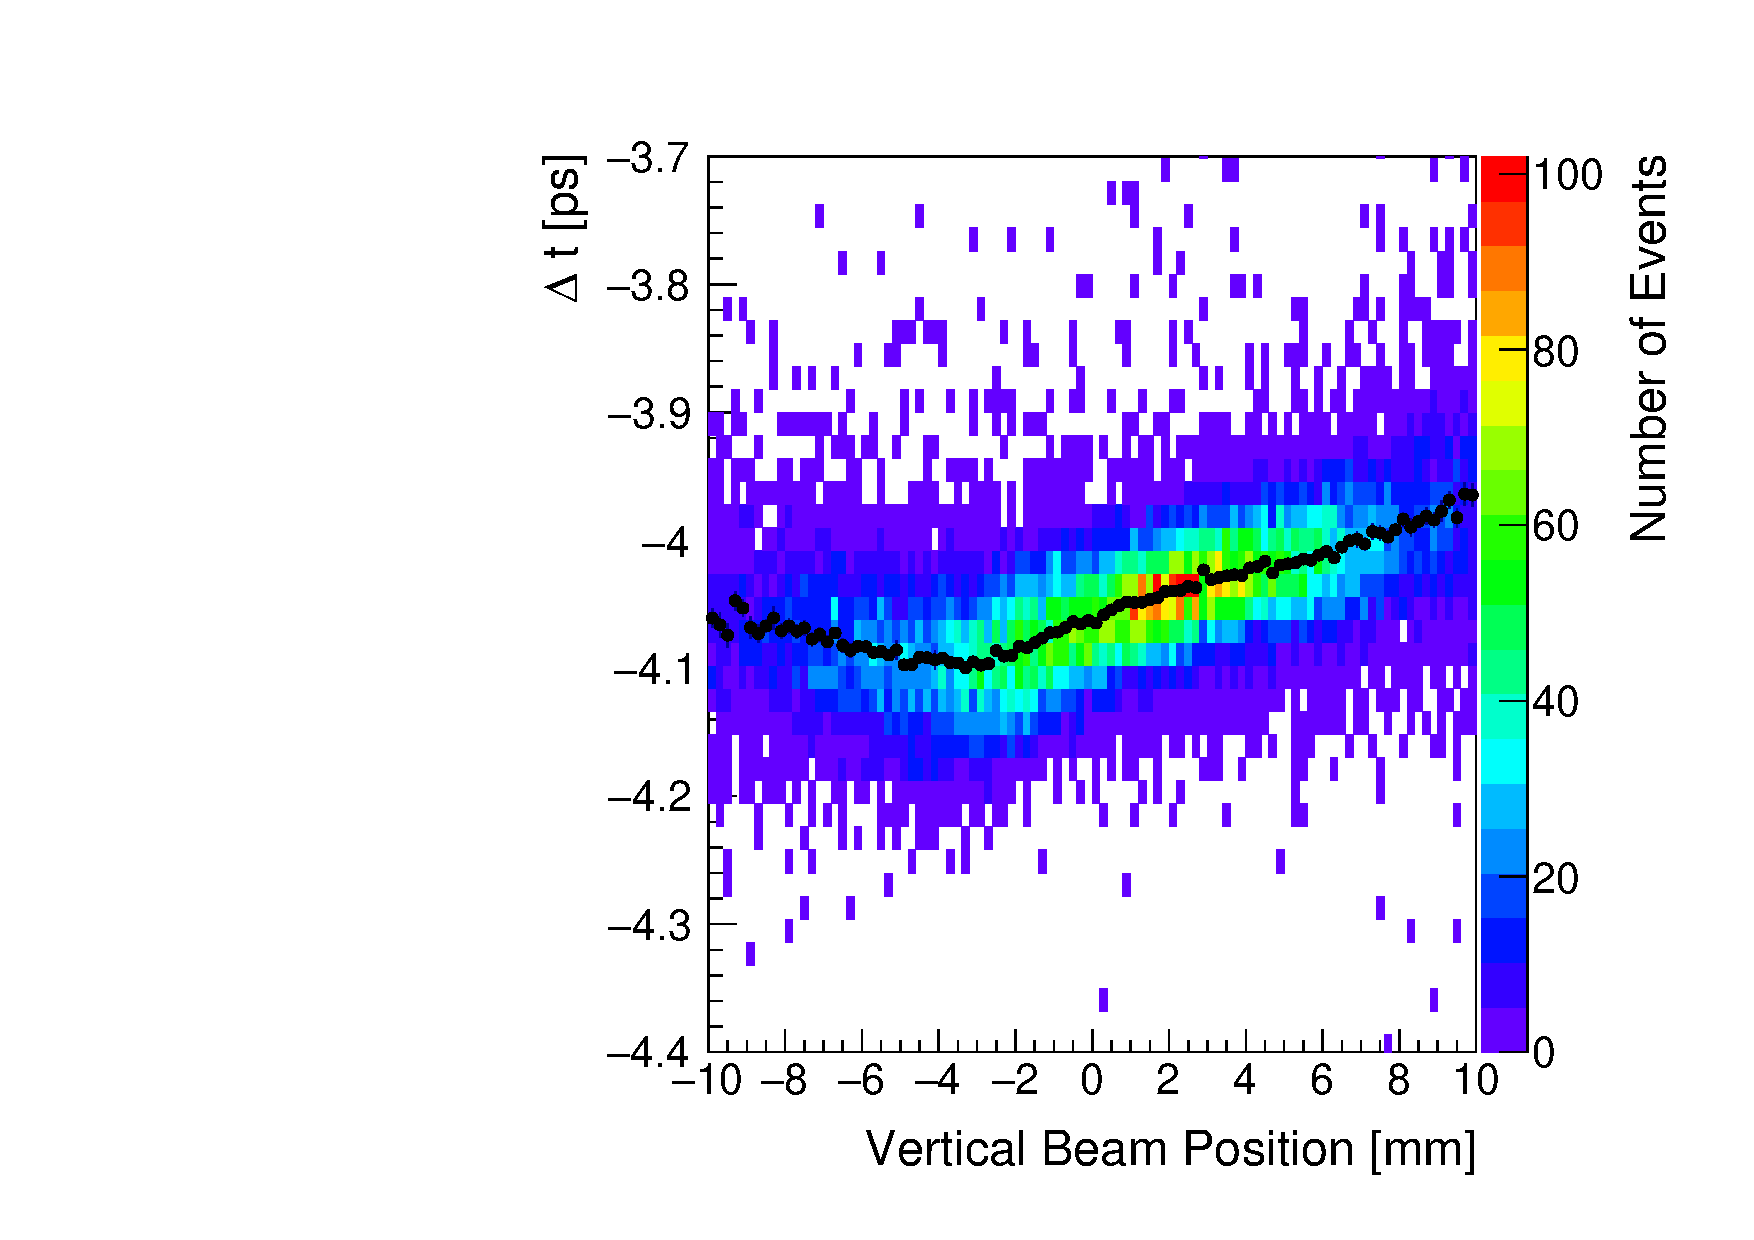
\includegraphics[width=0.49\textwidth]{figures/DeltaTVsVerticalPosition.pdf} 
\caption{ The distribution of the beam particle position measured by the wire chamber
and the time measured in the CdTe sensor relative to the Photek reference detector
is shown in the color scale. The mean value of the time measured in the CdTe sensor as a function
of the beam particle position is shown in the black points. There is a dependence of the time difference
on the impact point on the CdTe sensor which corresponds to about 100 ps across the CdTe sensor.} 
\label{fig:DeltaTVsBeamXY} 
\end{figure} 

\begin{figure}[htbp] 
\centering
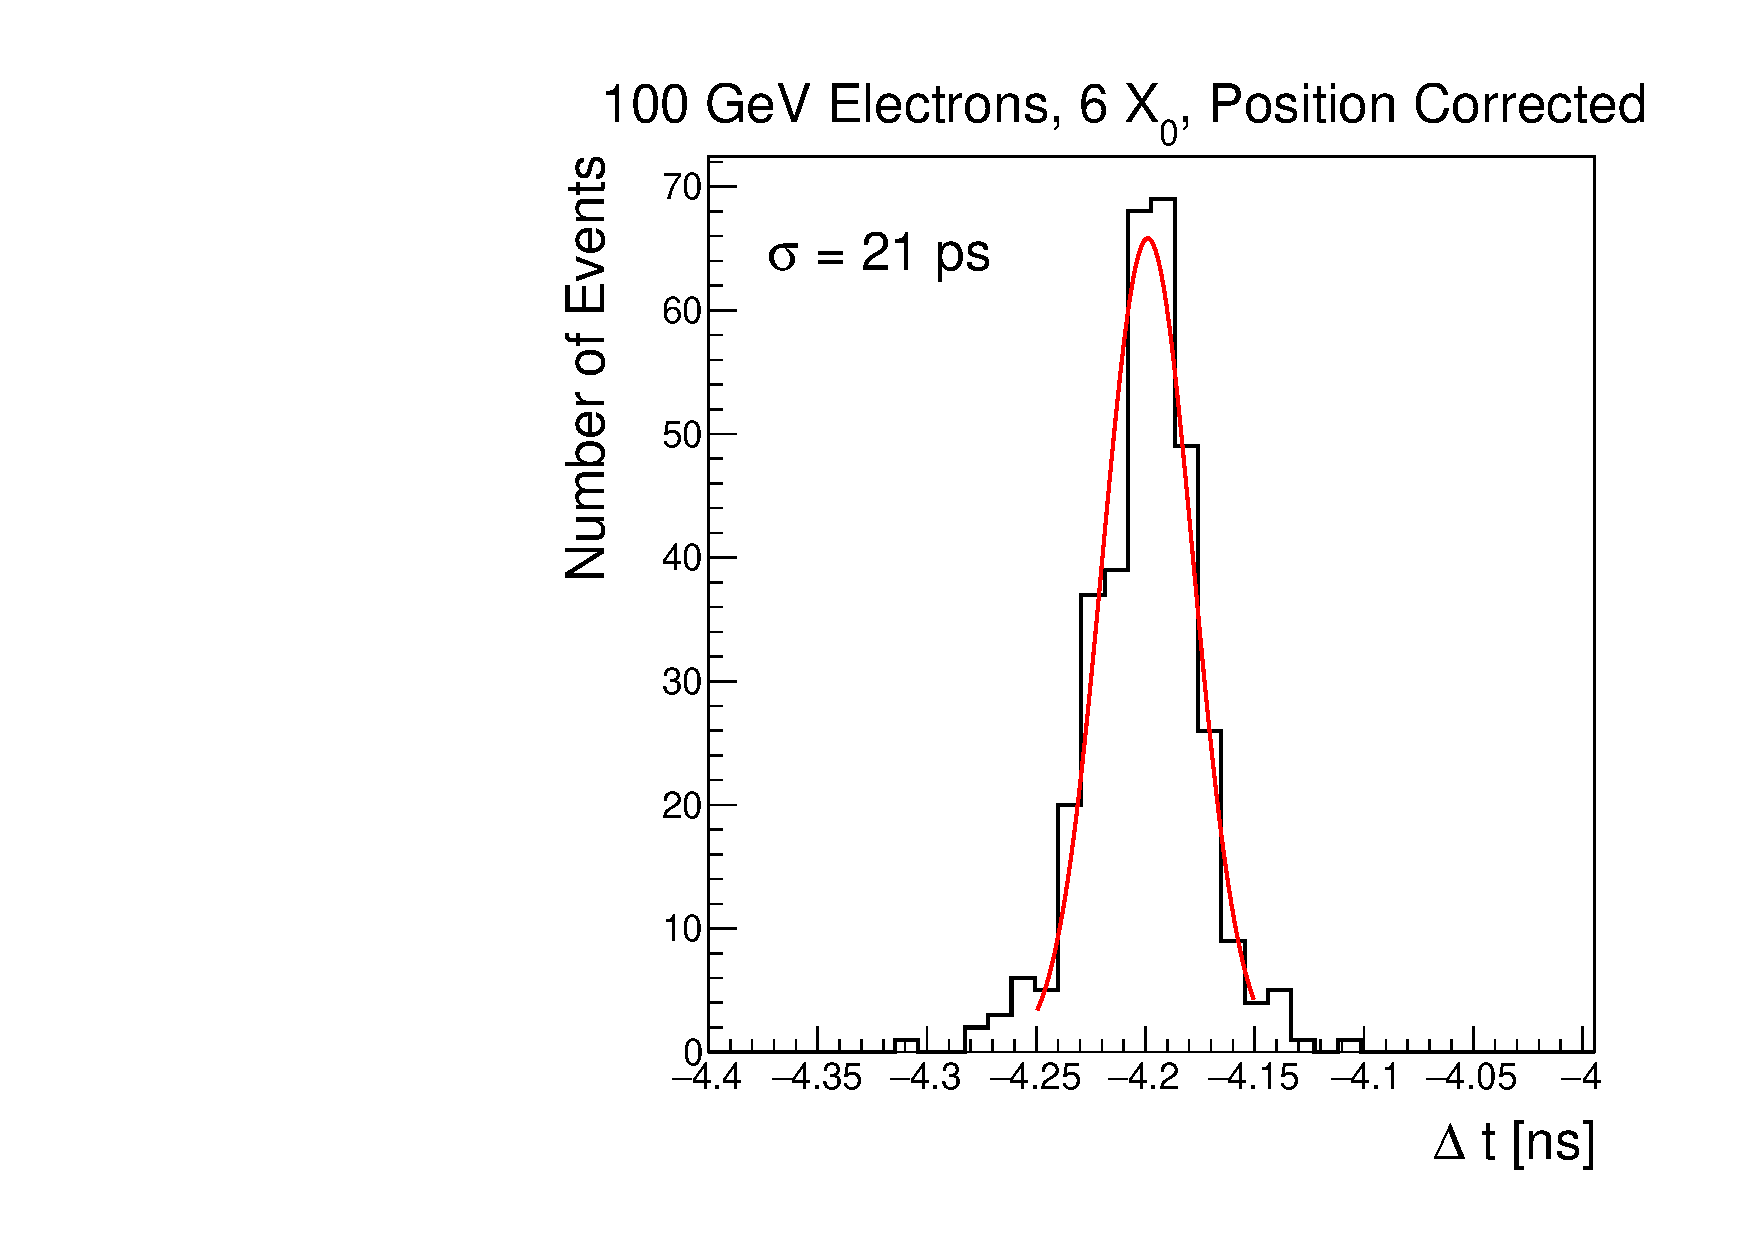
\includegraphics[width=0.49\textwidth]{figures/CdTeTimingResolution_100GeV_PositionCorrected.pdf} 
\caption{Distribution of the time-stamp measurement corrected for the geometric position
non-uniformity in the CdTe sensor for a $100$~GeV electron after $6$~$\mathrm{X}_{0}$ of tungsten absorber. } 
\label{fig:DeltaTCorr} 
\end{figure} 



%Figure: Time Resolution vs Beam Location
\begin{figure}[htbp] 
\centering
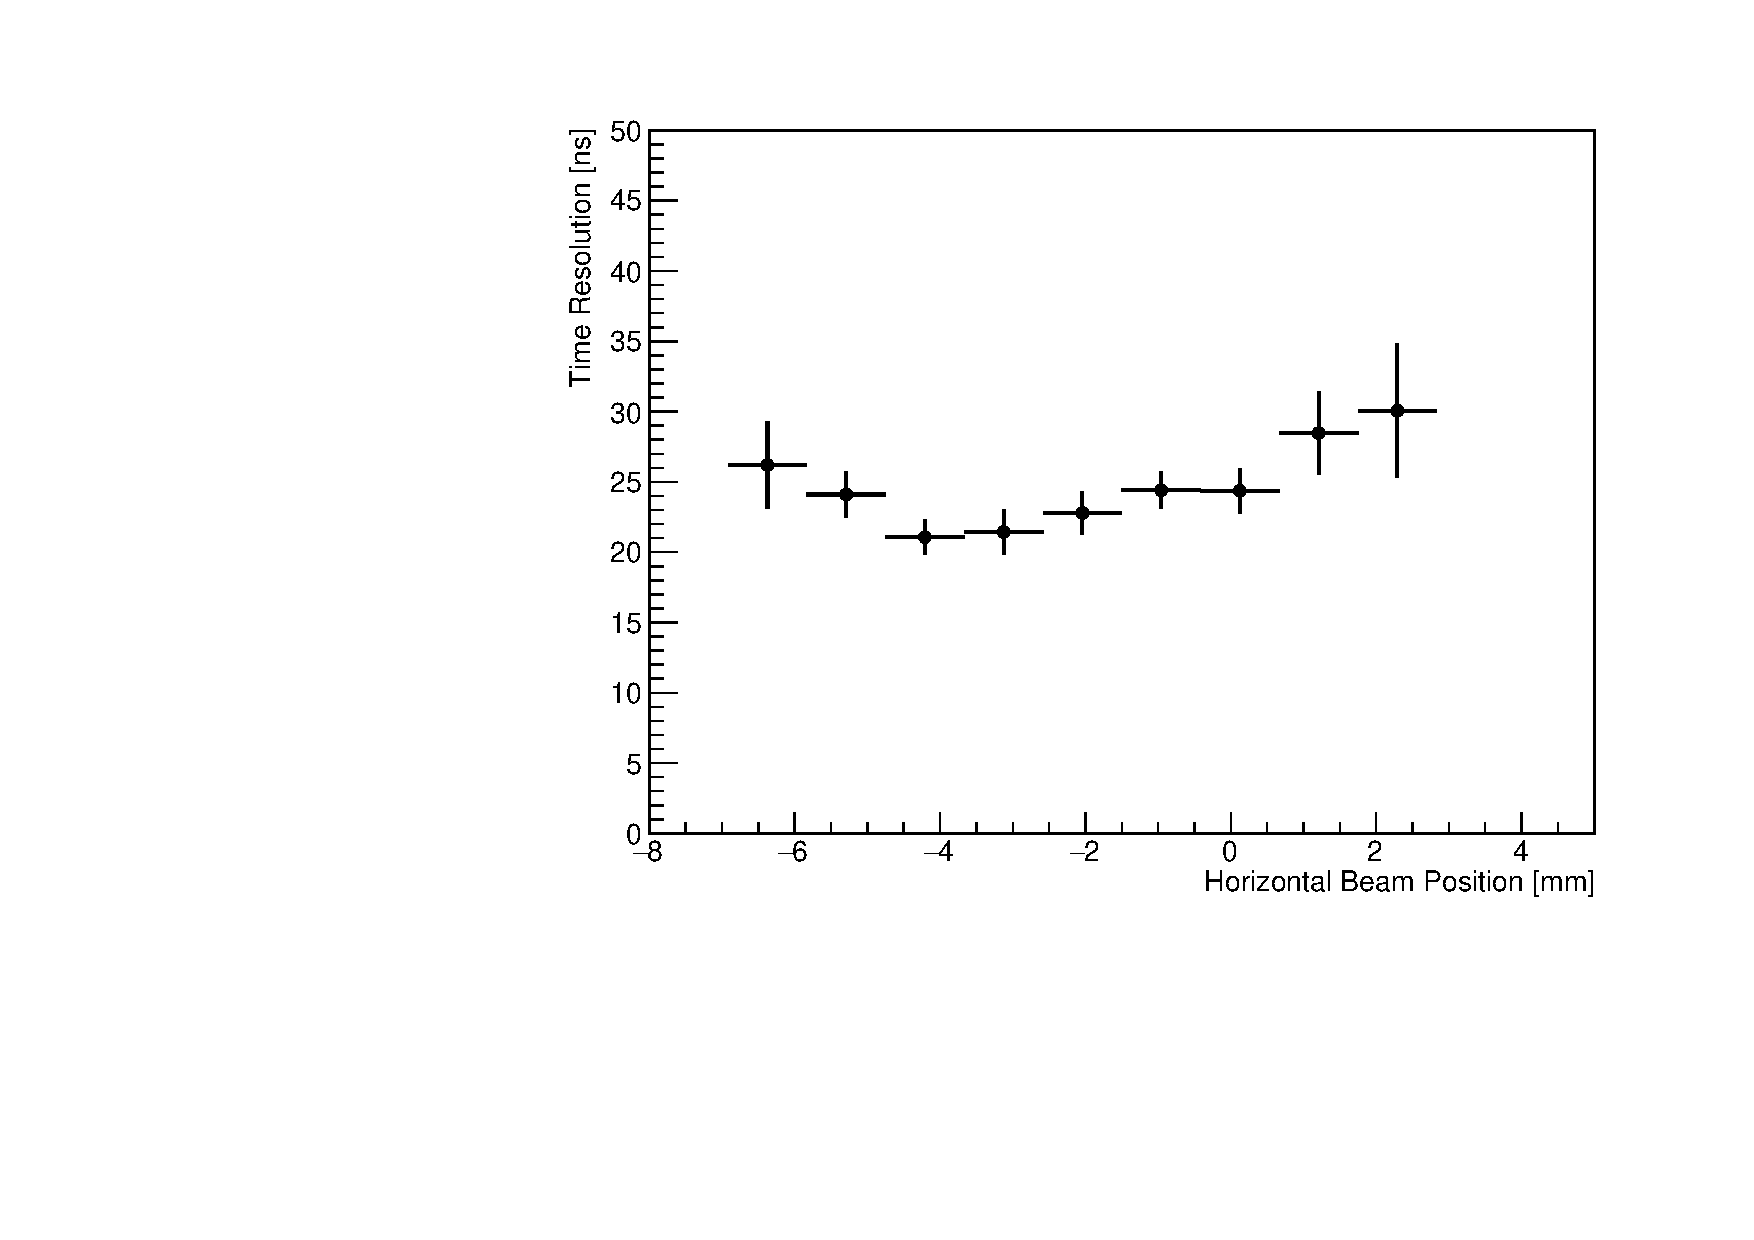
\includegraphics[width=0.49\textwidth]{figures/TimeResolutionVsBeamHorizontalPosition.pdf} 
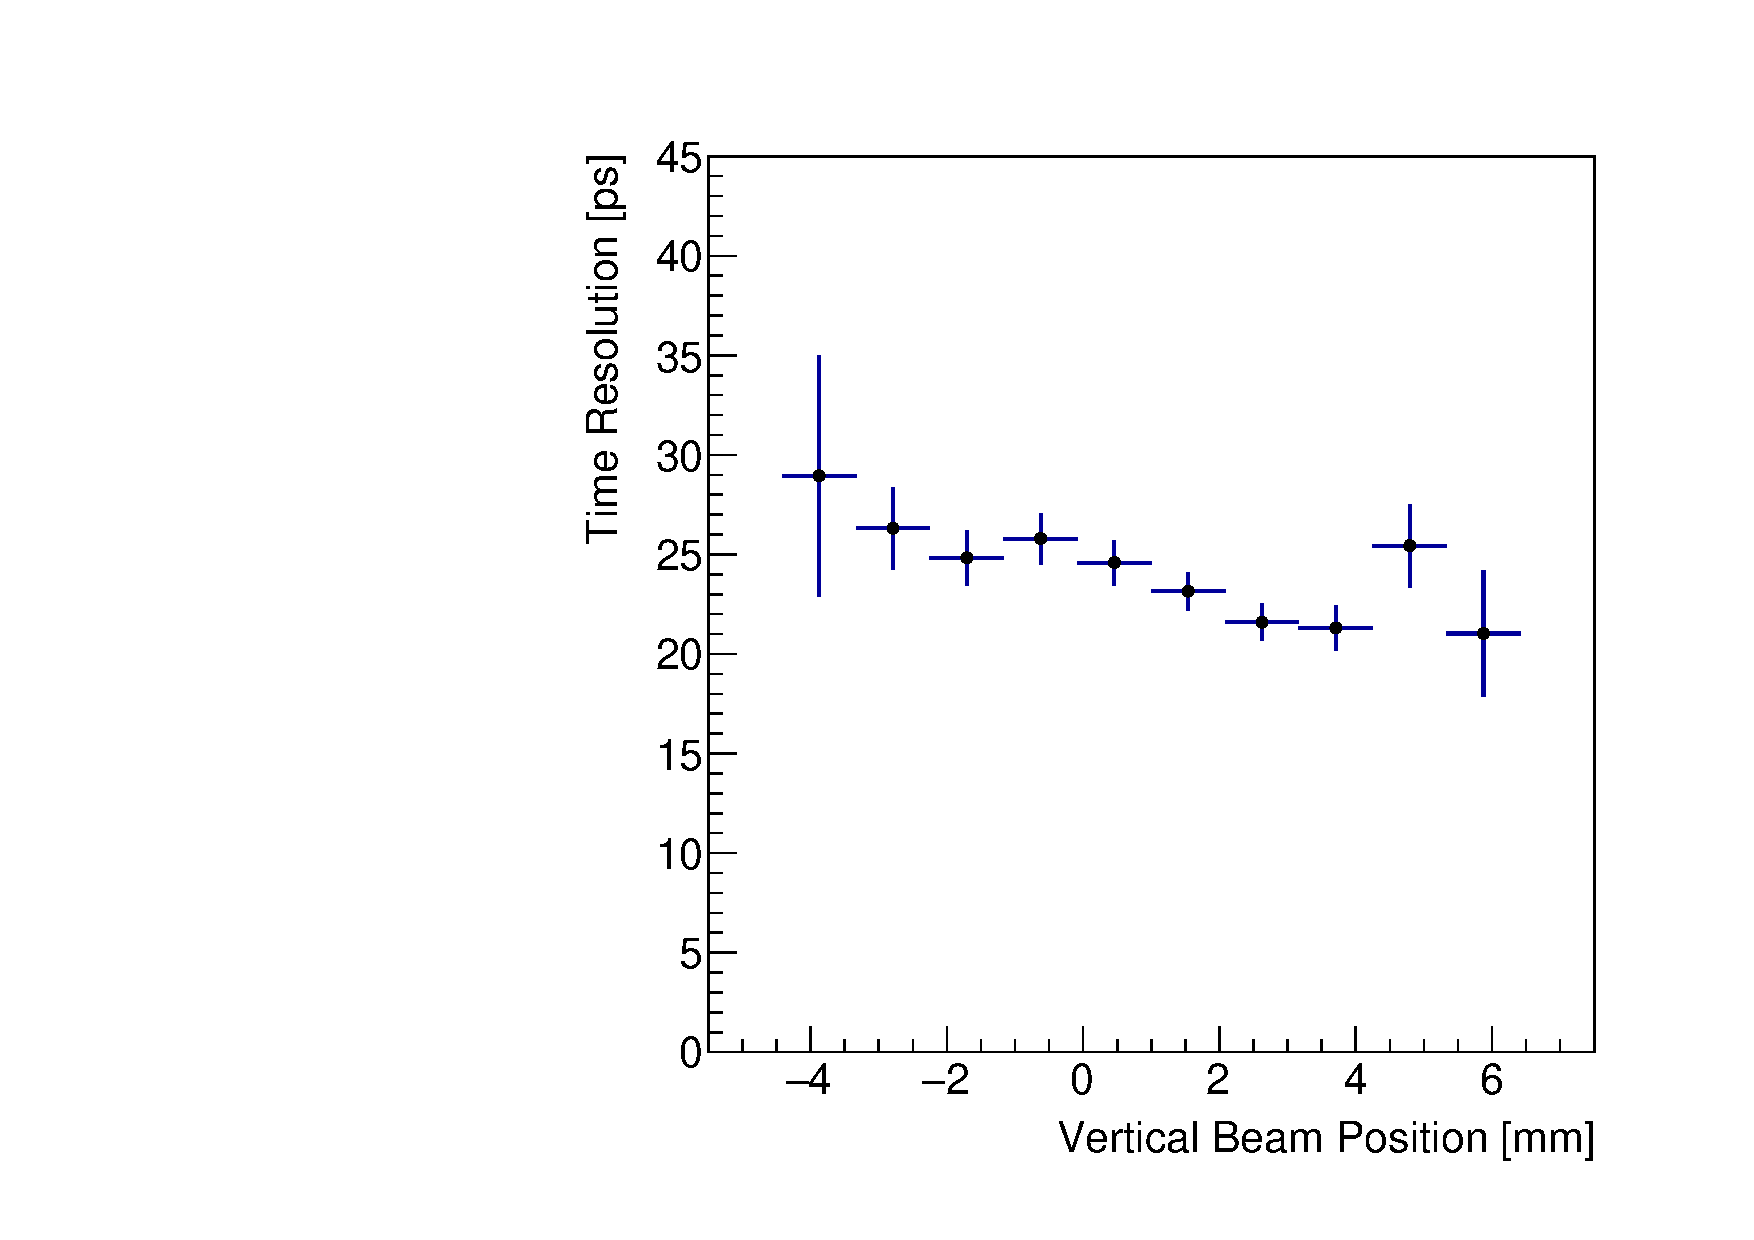
\includegraphics[width=0.49\textwidth]{figures/TimeResolutionVsBeamVerticalPosition.pdf} 
\caption{ The time resolution is measured as a function of the horizontal (left) and vertical (right)
beam position in a 2 mm wide region around the center of the sensor in the vertical (left) 
and horizontal (right) directions respectively. }
\label{fig:TimeResolutionVsBeamXY} 
\end{figure} 


%Figure: Time Resolution vs Anode Wire Bond Location  
\begin{figure}[htbp]
\centering 
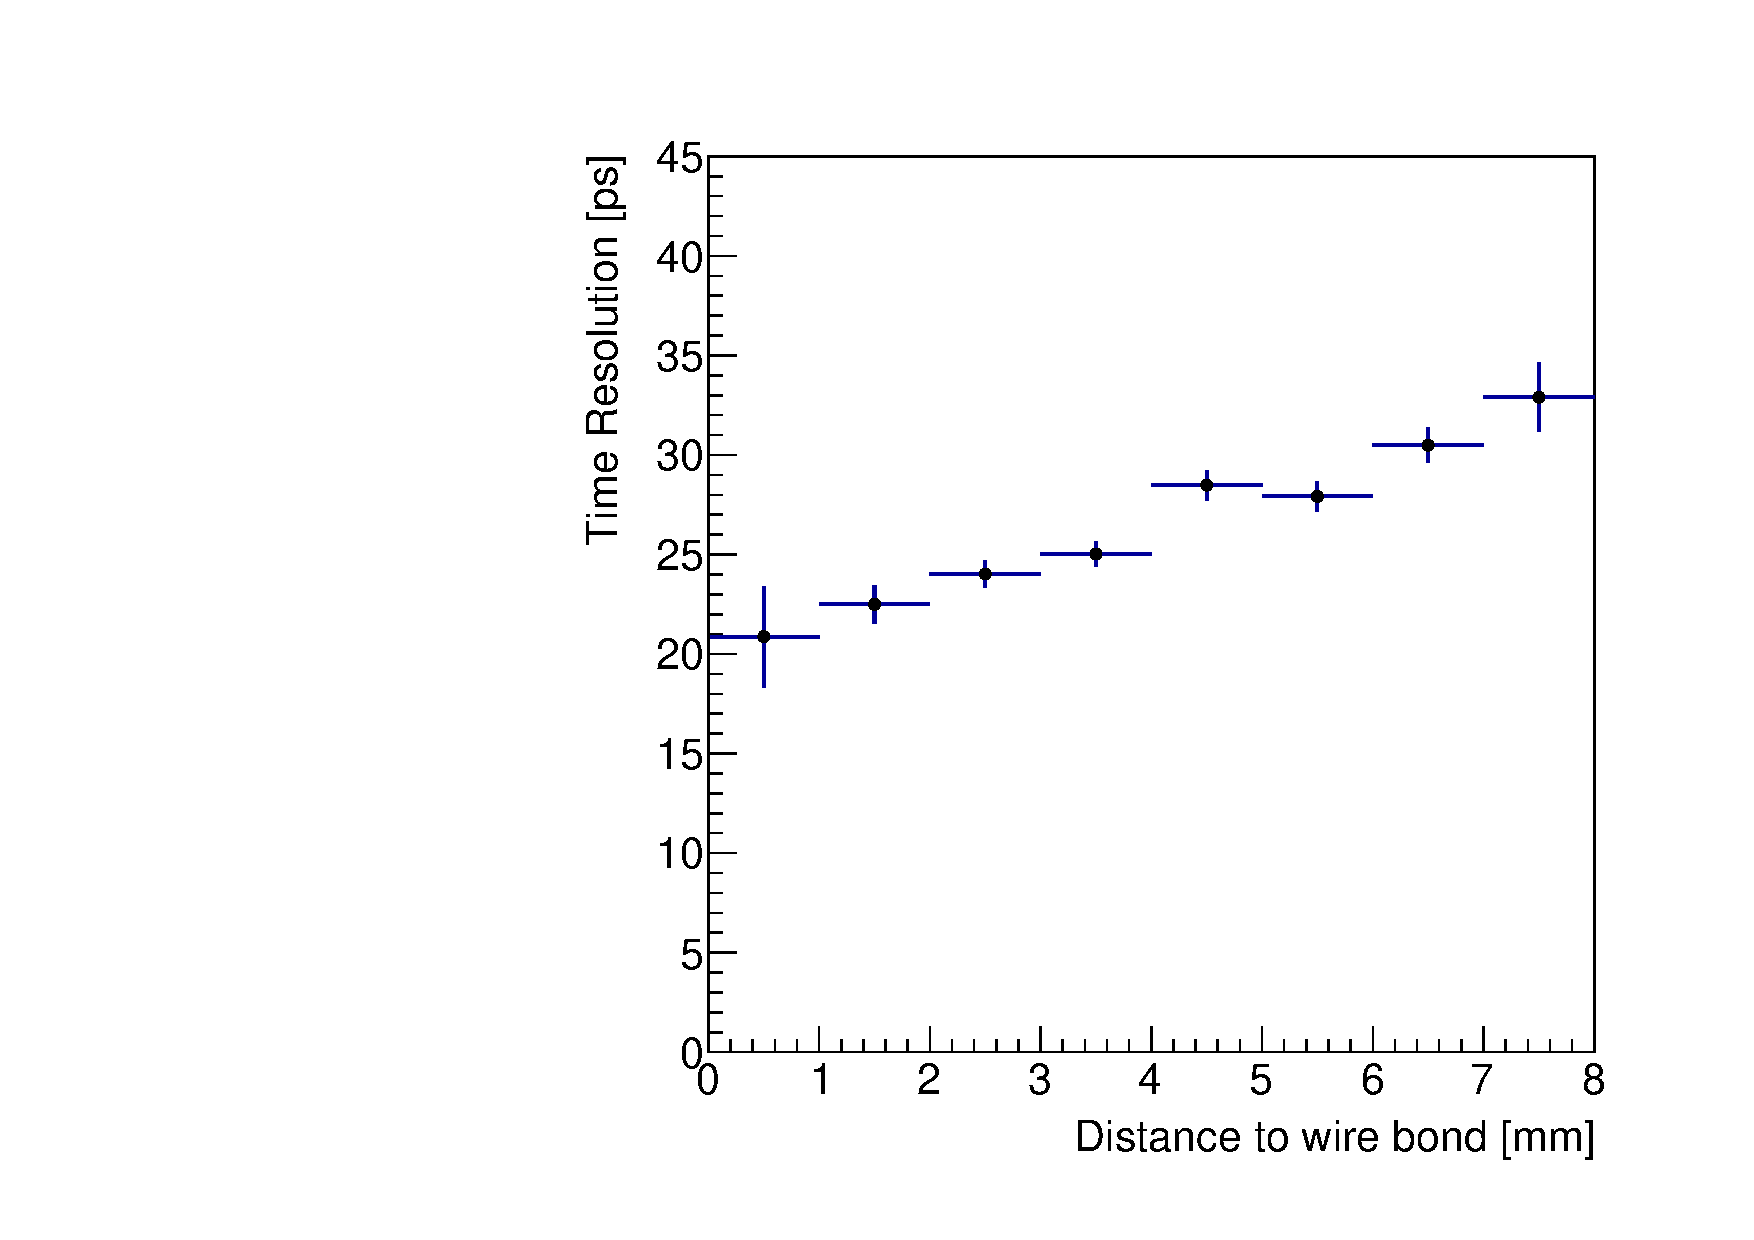
\includegraphics[width=0.49\textwidth]{figures/TimeResolutionVsR.pdf} 
\caption{ The time resolution is measured as a function of the planar distance of the 
incident beam particle to the back wire bond location on the sensor. The position non-uniformity
of the time response as shown in Figure~\ref{fig:DeltaTVsBeamXY} has been corrected for. There 
remains a dependence of the measured resolution across the sensor, reaching 20 ps in the location
closest to the back wire bond connection.}
\label{fig:TimeResolutionVsR}
\end{figure}




%Extra studies
%MIP peak
%Charge vs beam location ( can we say anything about signal size on shower periphery? )
  
%
%

\section{Discussion and Summary}
\label{sec:summary} 


In this article, we describe the first measurement of high energy 
electromagnetic showers using Cadmium-Telluride sensors. 
These initial results are encouraging and motivate future work on 
more detailed comparisons with simulation and more detailed 
measurements of transverse and longitudinal shower profiles.


%The energy loss per $\mathrm{g}/\mathrm{cm}^{3}$ mass density 
%for a minimum ionizing particle (MIP) is $1.26$~MeV$\mathrm{g}^{-1}\mathrm{cm}^{2}$ 
%for CdTe. For Silicon it is $1.66$~MeV$\mathrm{g}^{-1}\mathrm{cm}^{2}$~\cite{PDG}. 
%For CdTe, with a density of $5.86\mathrm{g}/\mathrm{cm}^{3}$, the energy
%loss is $0.74$~keV/$\mu$m. The mean energy to produce an electron hole pair
%in CdTe is $4.43$~eV~\cite{Sze,Singh}, resulting in a signal size of
%167 electron hole pairs per $\mu$m thickness per MIP, or $27$~fC/mm per
%MIP. This signal size for the CdTe sensor is a factor of $1.55$ larger per unit thickness
%than for silicon sensors. 
%Based on Figure~\ref{figures/ChargeVsEnergyAt6X0.pdf}, we project that at 32~GeV after $6$~$X_{0}$ 
%of absorber, the total charge collected is $2.3$~pC, which amounts to about $85$ MIP-equivalent
%signals. This is larger than the measured value of $54$ for silicon sensors under the same
%beam energy and absorber thickness conditions. The extra signal may be a result of additional
%sensitivity to keV range photons produced in the electromagnetic shower.

We have measured the rise time for signals in the Schottky type CdTe sensor diode to be about $1.35$~ns, which
is relatively fast and suggests that there is potential for precision timing.
We observe dependencies of the measured time on the geometric position of the
beam particle, which may indicate differences in the charge collection path.
More detailed studies of this aspect are needed and a more optimal design of the 
readout system is possible. Correcting for these dependencies yield time resolutions
of $25$~ps for a single layer CdTe sensor of transverse area $1$~cm~$\times$~$1$~cm
sampling the electromagnetic shower of electrons with energy above $100$~GeV 
after $6$ radiation lengths of tungsten and lead absorber. These initial results are encouraging and motivate 
further in-depth studies in the future.


%% The Appendices part is started with the command \appendix;
%% appendix sections are then done as normal sections
%% \appendix

%% \section{}
%% \label{}
  


\section{Acknowledgments} 
Supported by funding from California Institute of Technology High Energy Physics
under Contract DE-SC0011925 with the United States Department of Energy. We
thank the CERN test-beam facilities personnel for excellent beam conditions 
during our test-beam time. We also thank Paolo Meridiani and Francesco Micheli
for their kind assistance on the setup of the DAQ system.


%
%
%% If you have bibdatabase file and want bibtex to generate the
%% bibitems, please use
%%
%%  \bibliographystyle{elsarticle-num} 
%%  \bibliography{<your bibdatabase>}

%% else use the following coding to input the bibitems directly in the
%% TeX file.

\bibliography{CdTeDetector}{}
\bibliographystyle{ieeetr} 

%\begin{thebibliography}{00}

%% \bibitem{label}
%% Text of bibliographic item

%\bibitem{}

%\end{thebibliography}

\end{document}
